\documentclass[UTF8,a4paper,12pt]{ctexbook} 

 \usepackage{graphicx}%学习插入图
 \usepackage{verbatim}%学习注释多行
 \usepackage{booktabs}%表格
 \usepackage{diagbox}
 \usepackage{geometry}%图片
 \usepackage{amsmath}
 \usepackage{amssymb}
 \usepackage{listings}%代码
 \usepackage{xcolor}  %颜色
 \usepackage{enumitem}%列表格式
 \usepackage{tcolorbox}
 \usepackage{algorithm}  %format of the algorithm
 \usepackage{algorithmic}%format of the algorithm
 \usepackage{multirow}   %multirow for format of table
 \usepackage{longtable} 
 \usepackage{tabularx} 	%表格排版格式控制
 \usepackage{array}	%表格排版格式控制
 \usepackage{hyperref} %超链接 \url{URL}
 % \setCJKmainfont{方正兰亭黑简体}  %中文字体设置
 % \setCJKsansfont{华康少女字体} %设置中文字体
 % \setCJKmonofont{华康少女字体} %设置中文字体

 \CTEXsetup[format+={\flushleft}]{section}

 \geometry{left=1.6cm,right=1.8cm,top=2cm,bottom=1.7cm} %设置文章宽度
 %%%% 设置图片目录
 \graphicspath{{figure/}}
 
 
 \pagestyle{plain} 		  %设置页面布局

 %代码效果定义
 \definecolor{mygreen}{rgb}{0,0.6,0}
 \definecolor{mygray}{rgb}{0.5,0.5,0.5}
 \definecolor{mymauve}{rgb}{0.58,0,0.82}
 \lstset{ %
 	backgroundcolor=\color{white},   % choose the background color
 	basicstyle=\footnotesize\ttfamily,      % size of fonts used for the code
 	%stringstyle=\color{codepurple},
 	%basicstyle=\footnotesize,
 	%breakatwhitespace=false,         
 	%breaklines=true,                 
 	%captionpos=b,                    
 	%keepspaces=true,                 
 	%numbers=left,                    
 	%numbersep=5pt,                  
 	%showspaces=false,                
 	%showstringspaces=false,
 	%showtabs=false,        
 	columns=fixed,
 	breaklines=true,                 % automatic line breaking only at whitespace
 	captionpos=b,                    % sets the caption-position to bottom
 	tabsize=4,
 	commentstyle=\color{mygreen},    % comment style
 	escapeinside={\%*}{*)},          % if you want to add LaTeX within your code
 	keywordstyle=\color{blue},       % keyword style
 	xleftmargin=.06\textwidth, 
 	stringstyle=\color{mymauve}\ttfamily,     % string literal style
 	frame=L,
 	rulesepcolor=\color{red!20!green!20!blue!20},
 	% identifierstyle=\color{red},
 	language=sql,
 }
 \author{\kaishu 郑华}
 \title{\heiti MySQL 数据库学习笔记}
 
\begin{document}          %正文排版开始
 	\maketitle
\chapter{Mysql 配置与安装}
	\section{Mysql 架构}
		\url{https://www.cnblogs.com/andy6/p/6626848.html}
		
		<MySql 技术内幕>: \url{https://www.cnblogs.com/lay2017/p/9165203.html}
		
		\subsection{MySQL 层次结构}
			\begin{figure}[H]
				\centering
				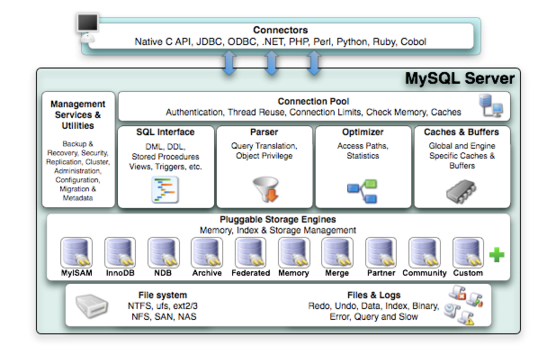
\includegraphics[width=17cm,height= 10cm]{arch}
				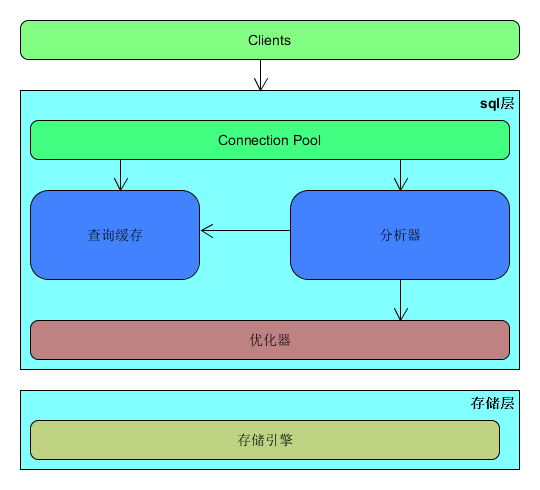
\includegraphics[width=16cm,height= 8cm]{arch2}			
				\caption{mysql 架构}
			\end{figure} 
			
			
			\begin{figure}[H]
				\centering
				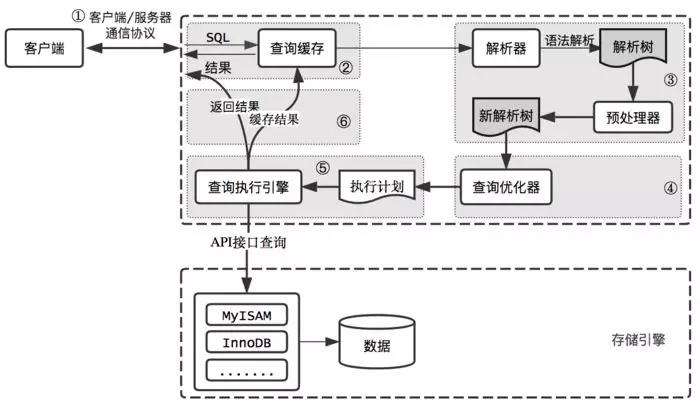
\includegraphics[width=16cm,height= 12cm]{mysqlArch2}
				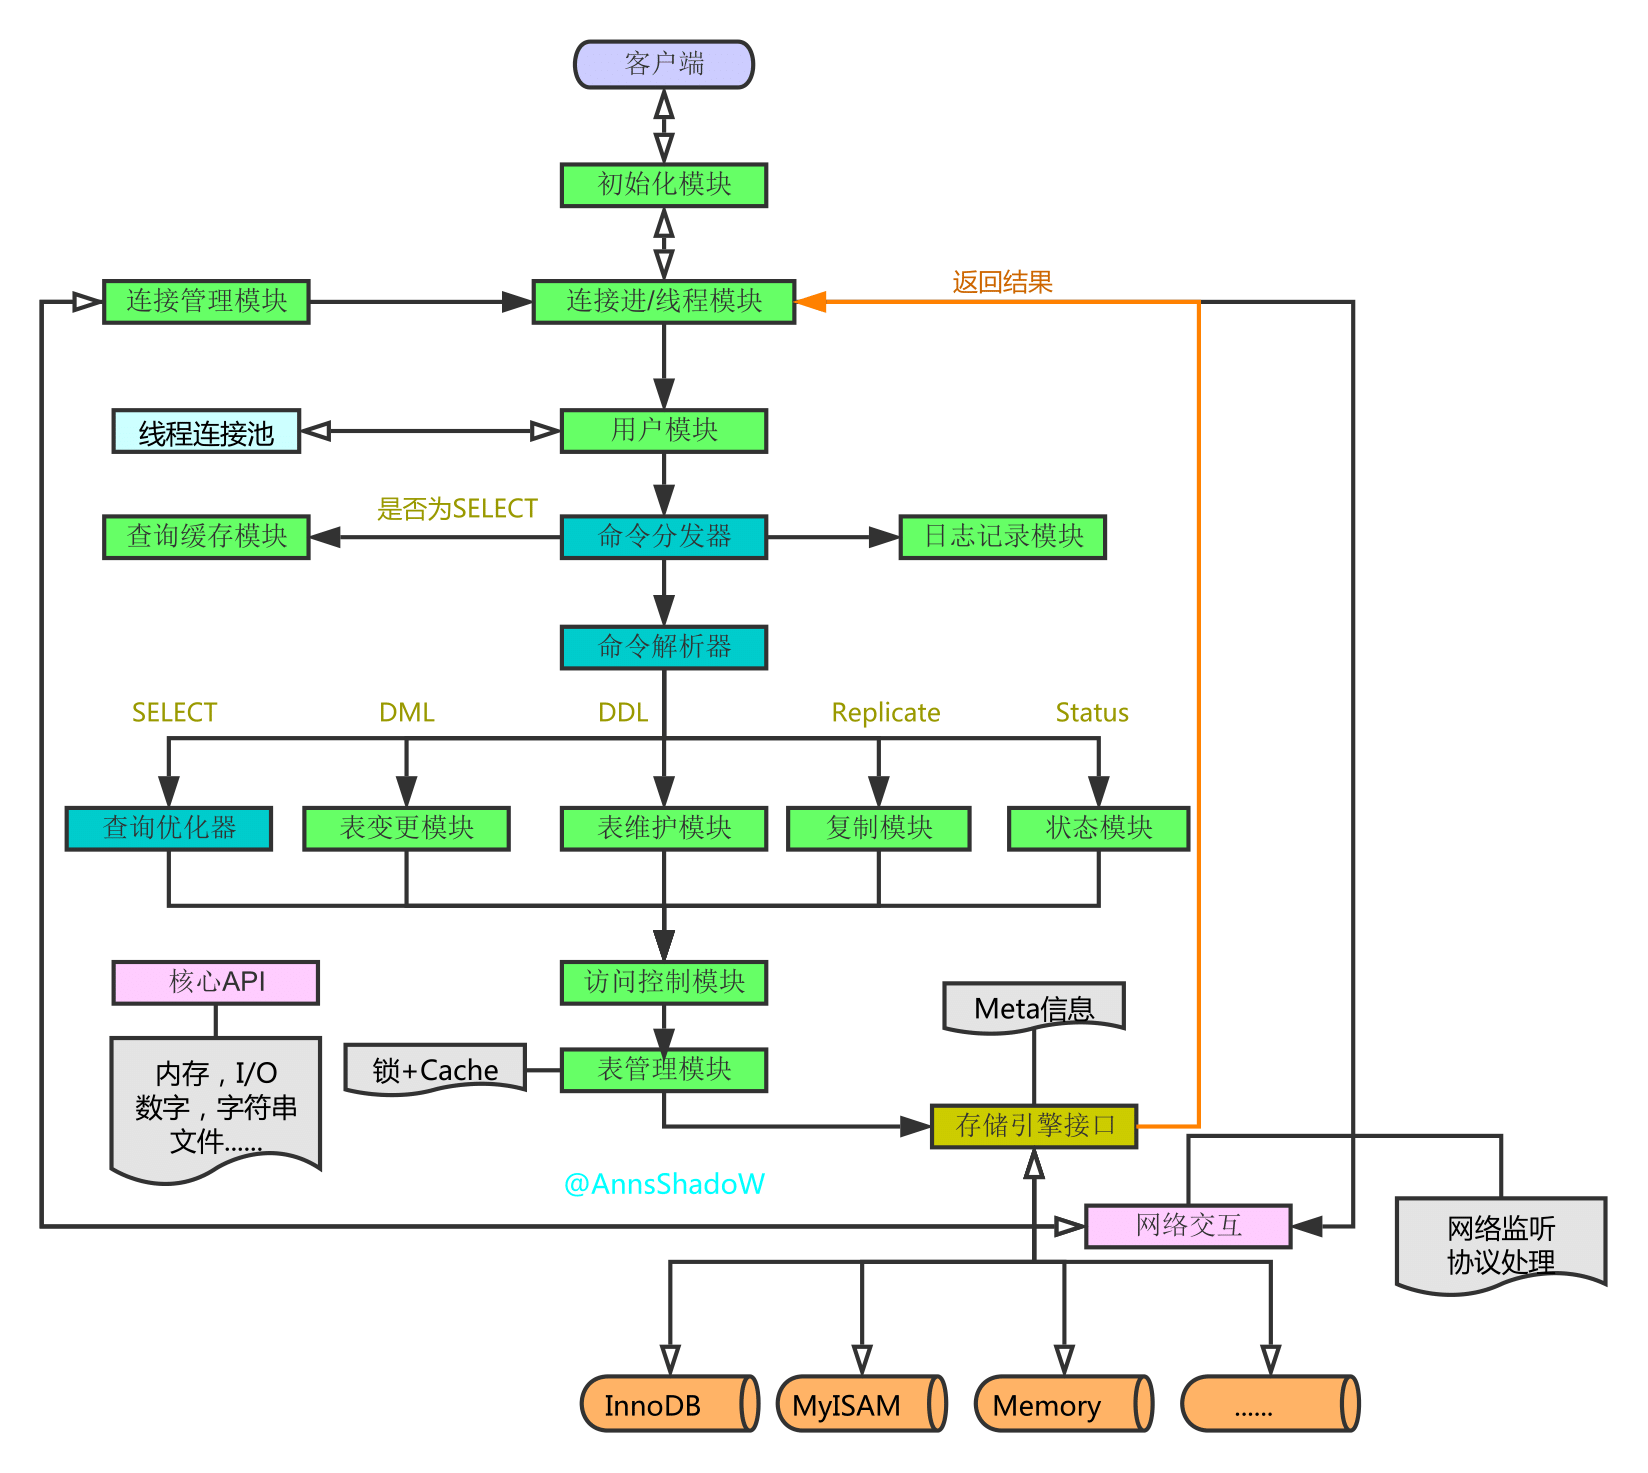
\includegraphics[width=17cm,height= 12cm]{mysqlArch}
				\caption{mysql 架构}
			\end{figure} 	
			
			
			\verb|Connectors|指的是不同语言中与SQL的交互。
			
			\verb|Management Serveices & Utilities|: 系统管理和控制工具。
			
			\verb|Connection Pool|: 连接池。管理缓冲用户连接,线程处理等需要缓存的需求。
			
			\verb|SQL Interface|: SQL接口。接受用户的SQL命令,并且返回用户需要查询的结果。比如select from就是调用SQL Interface。
			
			\verb|Parser|:解析器。SQL命令传递到解析器的时候会被解析器验证和解析。解析器是由Lex和YACC实现的,是一个很长的脚本。主要功能:
				\begin{itemize}[itemindent = 1em]
					\item 将SQL语句分解成数据结构,并将这个结构传递到后续步骤,以后SQL语句的传递和处理就是基于这个结构的。
					\item 如果在分解构成中遇到错误,那么就说明这个sql语句是不合理的。
				\end{itemize}
			
			\verb|Optimizer|: 查询优化器。
			
			\verb|Cache和Buffer|: 查询缓存。
				\begin{itemize}[itemindent = 1em]
					\item 如果查询缓存有命中的查询结果,查询语句就可以直接去查询缓存中取数据。这个缓存机制是由一系列小缓存组成的。比如表缓存,记录缓存,key缓存,权限缓存等。
				\end{itemize}
			
			\verb|Engine| :存储引擎。
					
			
			\verb|mysql|是一个\textbf{C/S架构模型},客户端通过与服务端建立连接来操作服务端数据;
			
			分析器\textbf{分析请求},并转发给优化器;
			
			通过缓存的方式提高查询性能;	
			
			优化器负责和底层的存储引擎进行交互,存储和查询mysql的数据;
		
		\subsection{物理文件组成}
			\begin{itemize}
				\item \textbf{日志文件}:
				\begin{itemize}
					\item \verb|Error log| 错误日志:记录遇到的所有严重的错误信息、每次启动关闭的详细信息;
					\item \verb|Binary log| 二进制日志:也就是binlog,记录所有修改数据库的操作;
					\item \verb|Query log| 查询日志:记录所有查询操作,体积较大,开启后对性能有影响;
					\item \verb|Slow Query log| 慢查询日志:记录所有执行时间超过\verb|long_query_time|的sql语句和达到\verb|min_examined_row_limit|条距离的语句;
					\item \verb|InnoDB redo log|:记录InnoDB所做的物理变更和事务信息;
				\end{itemize}
				
				\item \textbf{数据文件}:
				\begin{itemize}
					\item \verb|.frm文件|:表结构定义信息
					\item \verb|.MYD文件|:MyISAM引擎的数据文件;
					\item \verb|.MYI文件|:MyISAM引擎的索引文件;
					\item \verb|.ibd文件|和\verb|.ibdata文件|:\textbf{InnoDB的数据和索引};\verb|.ibdata|配置为共享表空间时使用,\verb|.ibd|配置为独享表空间时使用;
				\end{itemize}
				
				\item \textbf{其他文件}:
				\begin{itemize}
					\item \verb|系统配置文件|:\verb|/etc/my.cnf|
					\item \verb|pid文件|:存储自己的进程ID
					\item \verb|Unix Socket文件|:连接客户端使用
				\end{itemize}
			\end{itemize}
		
	\section{用户管理}
		\subsection{CREATE USER}
			创建用户
			
			\verb|CREATE USER  'userName' IDENTIFIED BY 'passwd';| 
			
		\subsection{GRANT}
			赋予用户权利
			
			\verb|GRANT ALL ON xxxdb.*  TO 'userName';| 
	
		
		\subsection{查看当前登录用户}
		
			\verb|select user();|
			
			类似的,查看当前使用的库是哪个,可以使用\verb|select database();|
			
	\section{建立和断开Mysql服务器连接}
		\verb|mysql options|
		
		\begin{itemize}[itemindent = 1em]
			\item \verb|-h |另一种形式是\verb|--host=host_name|
			\item \verb|-p |另一种形式是\verb|--password|
			\item \verb|-u |另一种形式是\verb|--user=user_name|
		\end{itemize}
		
			其余选项可以通过\verb|mysql --help|进行查看。
				
			为了避免在每次连接数据库的时候都需要对连接参数进行设定(主机名、用户名、密码等),有以下2种常用方式简化输入。
			
		\subsection{简化链接- 选项文件}
			\verb|client| 参考客户端配置。
		
		\subsection{简化连接- shell 别名}
			\verb|alias| 
		
		
	
	\newpage
	\section{Mysql 配置说明-my.cnf my.ini}
		
		\subsection{客户端的参数}
			下面显示的是客户端的参数,\verb|[client]|和\verb|[mysql]|都是客户端,下面是参数简介:
			
			\begin{table}[H]
				\centering
				\caption{客户端配置}
				\begin{tabular}{p{5cm}<{\centering}|p{12cm}<{\centering}}
					\toprule
						参数 &  含义 \\
					\midrule
						\verb|port=3306  | & 表示的是MySQL数据库的端口 \\
						\verb|default-character-set | & 是客户端默认的字符集,如果你希望它支持中文,可以设置成gbk或者utf8 \\
						\verb|user| & 在这里设置用户名\\
						\verb|password | & 在这里设置了password参数的值就可以在登陆时不用输入密码直接进入 \\
					\bottomrule
				\end{tabular}
			\end{table}	
			
			\begin{lstlisting}
# CLIENT SECTION
[client]

port=3306
user=testUserName
password=secret

[mysql]

default-character-set=gb2312			
			\end{lstlisting}
		
		\newpage
		\subsection{服务端的参数}	
			下面显示的是服务端的参数,\verb|[mysqld]|,下面是参数简介:
			
			\begin{table}[H]
				\centering
				\caption{常用配置说明}
				\begin{tabular}{p{8cm}<{\centering}|p{10cm}<{\centering}}
					\toprule
						参数 &  含义 \\
					\midrule
						\verb|basedir=.../mysql  | &  表示MySQL的安装路径 \\
						\verb|datadir=.../mysql/data  | & 表示MySQL数据文件的存储位置,也是数据库表的存放位置 \\
						\verb|port=3306  | & 端口 \\
						\verb|default-character-set |& 表示默认的字符集,这个字符集是服务器端的。\\
						\verb|default-storage-engine=INNODB  | & 设置服务器默认的存储引擎 \\
						\verb|sql-mode |& 表示SQL模式的参数,通过这个参数可以设置检验SQL语句的严格程度。\\
						\verb|server_id =111  | & 实例ID,主从时需要区分 \\
						\verb|log_bin =.../log/mysql-bin  | &  二进制日志文件名\\
						\verb|log_bin_index=.../log/mysql-bin.index  | & 二进制日志文件索引目录 \\
						\verb|max_binlog_size=200M  | &  \\
						\verb|binlog_format=ROW  | & binlog的格式 \\
						\verb|expire_logs_days=7  | &  二进制日志自动删除的天数。 \\
						\verb|slow_query_log=1  | & 慢查询日志的开启,默认为0,不开启 \\
						\verb|slow_query_log_file=.../slow.log  | & 慢查询日志文件路径 \\
						\verb|long_query_time =3  | & 查询时间超过设定的值,就会写入慢查询日志,方便语句的优化排查 \\
						\verb|general_log=1  | &  执行日志开启,默认关闭,不介意开启。\\
						\verb|general_log_file=.../log/mysql.log  | & 全局执行日志文件路径,记录了操作sql的完整记录。 \\
						\verb|log-error=.../log/mysql-error  | &  错误日志的文件路径\\
						\verb|log_output=table,file  | & 日志输出方式,默认为file,table的形式增加了服务器的压力,但方便在线通过语句\verb|SELECT|查询慢查询记录 \\
						\verb|event_scheduler=on  | & 设置事件的开启,自带的定时任务 \\
						\verb|interactive_timeout=28800  | & 设置sleep的断开时间,默认为86400(24小时),单纯的设置\verb|wait_timeout|无效 \\
						\verb|log-bin-trust-function-creators=1  | &不区分大小写  \\
						\verb|log_timestamps=SYSTEM  | & 日志文件时区跟随系统 \\	
						\verb|skip-name-resolve  | & 禁止MySQL对外部连接进行DNS解析 \\				
						\verb|back_log = 600  | & MySQL能有的连接数量。 \\
						\verb|max_connections = 1000  | & MySQL的最大连接数 \\
						\verb|max_connect_errors = 6000  | &  \\
						\verb|open_files_limit = 65535  | & MySQL打开的文件描述符限制,默认最小1024. \\								
					\bottomrule
				\end{tabular}
			\end{table}
			
			\begin{table}[H]
				\centering
				\caption{常用配置说明(续1)}
				\begin{tabular}{p{6cm}<{\centering}|p{12cm}<{\centering}}
					\toprule
						参数 &  含义 \\
					\midrule
						\verb|max_allowed_packet=32M  | & 接受的数据包大小 \\
						\verb|table_open_cache = 128  | & MySQL每打开一个表,都会读入一些数据到\verb|table_open_cache|缓存中,默认值64。 \\	
						\verb|binlog_cache_size= 1M  | & 一个事务,在没有提交的时候,产生的日志,记录到Cache中;等到事务提交需要提交的时候,则把日志持久化到磁盘。 \\
						\verb|max_heap_table_size = 8M  | & 定义了用户可以创建的内存表(memory table)的大小。这个值用来计算内存表的最大行数值。这个变量支持动态改变 \\
						\verb|tmp_table_size = 16M  | & MySQL的heap(堆积)表缓冲大小。 \\
						\verb|read_buffer_size = 2M  | & MySQL读入缓冲区大小。 \\
						\verb|read_rnd_buffer_size = 8M  | & MySQL的随机读缓冲区大小。 \\
						\verb|sort_buffer_size = 8M  | & 执行排序使用的缓冲大小。 \\
						\verb|join_buffer_size = 8M  | & 联合查询操作所能使用的缓冲区大小 \\
						\verb|thread_cache_size = 8  | & 这个值(默认8)表示可以重新利用保存在缓存中线程的数量,当断开连接时如果缓存中还有空间,那么客户端的线程将被放到缓存中 \\
						\verb|query_cache_size = 8M  | & MySQL的查询缓冲大小 \\
						\verb|query_cache_limit = 2M | & 指定单个查询能够使用的缓冲区大小,默认1M\\
						\verb|key_buffer_size = 4M | & 指定用于索引的缓冲区大小,增加它可得到更好处理的索引(对所有读和多重写),到你能负担得起那样多。\\
						\verb|transaction_isolation = | & 4种事务隔离级别\\
					\bottomrule
				\end{tabular}
			\end{table}
			
			\begin{lstlisting}
# SERVER SECTION

[mysqld]

# The TCP/IP Port the MySQL Server will listen on
port=3306


#Path to installation directory. All paths are usually resolved relative to this.
basedir="E:/Java/Mysql/"

#Path to the database root
datadir="C:/ProgramData/MySQL/MySQL Server 5.5/Data/"

# The default character set that will be used when a new schema or table is
# created and no character set is defined
character-set-server=gb2312

# The default storage engine that will be used when create new tables when
default-storage-engine=INNODB

# Set the SQL mode to strict
sql-mode="STRICT_TRANS_TABLES,NO_AUTO_CREATE_USER,NO_ENGINE_SUBSTITUTION"			
			\end{lstlisting}
		
		\verb|sql-mode|: 表示SQL模式的参数,通过这个参数可以设置检验SQL语句的严格程度。如果sql 语句正确,结果错误,一般都是\verb|sql_mode| 设置的问题。
		\url{https://www.cnblogs.com/zhengbin/p/5874906.html}
					
		\verb|back_log |:\textbf{当主要MySQL线程在一个很短时间内得到非常多的连接请求,这就起作用},然后主线程花些时间(尽管很短)检查连接并且启动一个新线程。\verb|back_log|值指出在MySQL暂时停止回答新请求之前的短时间内多少个请求可以被存在堆栈中。如果期望在一个短时间内有很多连接,你需要增加它。也就是说,如果MySQL的连接数据达到\verb|max_connections|时,新来的请求将会被存在堆栈中,以等待某一连接释放资源,该堆栈的数量即\verb|back_log|,如果等待连接的数量超过\verb|back_log|,将不被授予连接资源。另外,这值(\verb|back_log|)限于您的操作系统对到来的TCP/IP连接的侦听队列的大小。你的操作系统在这个队列大小上有它自己的限制(可以检查你的OS文档找出这个变量的最大值),试图设定\verb|back_log|高于你的操作系统的限制将是无效的。	
		
		
		\verb|max_binlog_size| : 如果当前的日志大小达到\verb|max_binlog_size|,还会自动创建新的二进制日志。如果你正使用大的事务,二进制日志还会超过\verb|max_binlog_size|:事务全写入一个二进制日志中,绝对不要写入不同的二进制日志中
		
		
		\verb|open_files_limit|: \textbf{MySQL打开的文件描述符限制},默认最小1024.当\verb|open_files_limit|没有被配置的时候,比较\verb|max_connections*5|和\verb|ulimit -n|的值,哪个大用哪个,当\verb|open_file_limit|被配置的时候,比较\verb|open_files_limit|和\verb|max_connections*5|的值,哪个大用哪个
		
		
		\verb|expire_logs_days|:  \textbf{二进制日志自动删除的天数}。默认值为0,表示“没有自动删除”。启动时和二进制日志循环时可能删除,根据实际业务需要与硬盘空间来决定。
		
		
		\verb|binlog_format|:binlog的格式也有三种:\verb|STATEMENT,ROW,MIXED|。默认为ROW
		
		\verb|general_log|: \textbf{执行日志开启,默认关闭},不介意开启。需要排查问题的通过在线执行set global \verb|general_log=ON|;开启,使用完后及时关闭通过\verb|set global general_log=OFF|;,占用的硬盘空间太大
		
		\verb|skip-name-resolve|: \textbf{禁止MySQL对外部连接进行DNS解析},使用这一选项可以消除MySQL进行DNS解析的时间。但需要注意,如果开启该选项,则所有远程主机连接授权都要使用IP地址方式,否则MySQL将无法正常处理连接请求
		
		\verb|transaction_isolation|: MySQL支持4种事务隔离级别,\verb|READ-UNCOMMITTED|, \verb|READ-COMMITTED|, \verb|REPEATABLE-READ|, \verb|SERIALIZABLE|。如没有指定,MySQL默认采用的是\verb|REPEATABLE-READ|,ORACLE默认的是\verb|READ-COMMITTED|
		
		\subsection{InnoDB 的参数}
			这个配置在服务端的选项下,\verb|[mysqld]|.
			
			\begin{table}[H]
				\centering
				\caption{INNODB 常用配置说明}
				\begin{tabular}{p{6cm}<{\centering}|p{12cm}<{\centering}}
					\toprule
						参数 &  含义 \\
					\midrule
						\verb|innodb_additional_mem_pool_size| & 表示附加的内存池,用来存储InnoDB表的内容。 \\
						\verb|innodb_flush_log_at_trx_commit| & 是设置提交日志的时机,若设置为1,InnoDB会在每次提交后将事务日志写到磁盘上 \\	
						\verb|innodb_log_buffer_size| & 表示用来存储日志数据的缓存区的大小 \\
						\verb|innodb_buffer_pool_size| & 表示缓存的大小,InnoDB使用一个缓冲池类保存索引和原始数据。 \\
						\verb|innodb_log_file_size| & 表示日志文件的大小 \\
						\verb|innodb_thread_concurrency| & 表示在InnoDB存储引擎允许的线程最大数 \\
					\bottomrule
				\end{tabular}
			\end{table}			
			
		
		
		\subsection{参考}	
			\url{https://www.2cto.com/database/201805/744792.html}
			
			\url{https://www.cnblogs.com/wyy123/p/6092976.html}	
	
	

		
	 \section{通识配置}	
	 	\subsection{服务器的 SQL Mode}
	 		\verb|sql_mode| 可以全局设置这个值这个变量,让它对所有客户端产生影响,也可以让每个客户端自己更改这个模式,从而只对其自己与他所连接的哪个服务器的会话产生影响。
	 		
	 		这意味着,任何客户端都可以在不影响其他客户端的前提下,更改服务器对待它自己的行为。
	 		
	 		如果想在启动前更改SQL模式,那么可以在MySQLd 的选项文件里配置 \verb|sql_mode|.
	 		
	 		如果想在运行时更改SQL模式,那么可以使用一条\verb|SET 语句| 来设置 \verb|sql_mode|系统变量。
	 		\begin{itemize}
	 			\item \verb|SET sql_mode = 'TRADATION'| 任何客户端为其自己设置一个本次会话特定的SQL模式。
	 			\item \verb|SET GLOBAL sql_mode = 'TRADATION'|	为所有客户端设置、或全局性的设置 SQL模式。
	 		\end{itemize}
	 		
	 		如果想知道当前会话或全局的SQL模式值,则可以使用如下语句:
	 		\begin{itemize}
	 			\item \verb|SELECT @@SESSION.sql_mode;|
	 			\item \verb|SELECT @@GLOBAL.sql_mode;|
	 		\end{itemize}
	 		
	 	\subsection{标识符语法 和 命名规则}
	 	
	 	
	 	\subsection{大小写规则}
	 		\begin{itemize}
	 			\item \textbf{SQL 关键字、函数名、列名、索引名} 不区分大小写。
	 			\item \textbf{数据库名、表名、视图名、存储过程名、别名}  区分大小写
	 		\end{itemize}
	 	
	 	\subsection{字符集支持}
		
		
	 \section{教程集合地址}
	 	\url{https://blog.csdn.net/orangleliu/article/details/54694272}
	 	
	 	DB入门笔记:\url{https://www.cnblogs.com/ggjucheng/archive/2012/11/02/2751119.html}
	 	
	 	\url{https://www.cnblogs.com/shockerli/p/1000-plus-line-mysql-notes.html}
	 	
\chapter{基本概念}
	 \section{术语}
		 \begin{itemize}
		 	\item  \textbf{数据库}: 数据库是一些关联表的集合。.
		 	\item  \textbf{数据表}: 表是数据的矩阵。在一个数据库中的表看起来像一个简单的电子表格。
		 	\item  \textbf{列}: 一列(数据元素) 包含了相同的数据, 例如邮政编码的数据。
		 	\item  \textbf{行}:一行(=元组,或\textbf{记录})是一组相关的数据,例如一条用户订阅的数据。
		 	\item  \textbf{冗余}:存储两倍数据,冗余降低了性能,但提高了数据的安全性。
		 	\item  \textbf{主键}:\textbf{主键是唯一的}。一个数据表中只能包含一个主键。你可以使用主键来查询数据。
		 	\item  \textbf{外键}:外键用于关联两个表。
		 	\item  \textbf{复合键}:复合键(组合键)将多个列作为一个索引键,一般用于复合索引。
		 	\item  \textbf{索引}:使用索引可快速访问数据库表中的特定信息。索引是对数据库表中一列或多列的值进行排序的一种结构。类似于书籍的目录。
		 	\item  \textbf{参照完整性}: 参照的完整性要求关系中不允许引用不存在的实体。与实体完整性是关系模型必须满足的完整性约束条件,目的是保证数据的一致性。
		 \end{itemize}
		
		\subsection{主键}
			一个主键比如:
			 
			\textbf{学生表(学号,姓名,性别,班级)} 其中每个学生的学号是唯一的,\textit{学号就是一个主键} 
			
			\textbf{课程表(课程编号,课程名,学分)} 其中课程编号是唯一的,\textit{课程编号就是一个主键} 
			
			\textbf{成绩表(学号,课程号,成绩)} 成绩表中单一一个属性无法唯一标识一条记录,学号和课程号的组合才可以唯一标识一条记录,所以 \textit{学号和课程号的属性组是一个主键} 
			
		\subsection{外键}
			定义在别的表存在的主键。
			
			接上:
			
			\underline{成绩表}中的\textbf{学号不是成绩表的主键},但它和学生表中的学号相对应,并且学生表中的学号是学生表的主键,\textit{则称成绩表中的学号是成绩表的外键} 
			  
			同理 成绩表中的\textbf{课程号}\textit{是成绩表的外键} 
			
			\url{https://blog.csdn.net/f45056231p/article/details/81070437}
			
			\begin{table}[H]
				\centering
				\caption{主键、外键、索引区别}
				\begin{tabular}{p{0.5cm}<{\centering}|p{5cm}<{\centering}|p{5.5cm}<{\centering}|p{4.5cm}<{\centering}}
					\toprule[1.5pt]
							 & 主键 	&  外键 &  索引\\
					\midrule
						定义 & 唯一标识一条记录,不能有重复的,不允许为空   & 表的外键是另一表的主键, 外键可以有重复的, 可以是空值      & 该字段没有重复值,但可以有一个空值  \\
						\hline
						作用 & 用来保证数据完整性   &  用来和其他表建立联系用的     & 是提高查询排序的速度  \\
						\hline
						个数 & 主键只能有一个   & 一个表可以有多个外键      & 一个表可以有多个惟一索引  \\
					\bottomrule[1.5pt]
				\end{tabular}
			\end{table}
			
		\subsection{参照完整性}
			\textbf{定义主键和外键}主要是\textbf{为了维护关系数据库的完整性},总结一下:
			
			\begin{itemize}
				\item \textbf{主键是能确定一条记录的唯一标识},比如,一条记录包括身份正号,姓名,年龄。\textbf{身份证号是唯一能确定}你这个人的,其他都可能有重复,所以,身份证号\textbf{是主键}。
				
				\item \textbf{外键用于与另一张表的关联}。是能确定另一张表记录的字段,用于保持数据的一致性。比如,A表中的一个字段,是B表的主键,那他就可以是A表的外键。
			\end{itemize}
		
			具体的参考:《MySQL 技术内幕 张雪平-译》 2.13
		\subsection{参考}
		
			系统博客:\url{https://www.cnblogs.com/geaozhang/category/1326927.html}
		
			周伯通博客:\url{https://www.cnblogs.com/phpper/tag/mysql/default.html?page=1}
	

	\section{SQL分类}
		\begin{itemize}
			\item 数据库查询:代表关键字 \verb|select|
			\item 数据库操纵:代表关键字 \verb|insert delete update|
			\item 数据库定义:代表关键字 \verb|create drop alter|
			\item 事务控制:代表关键字 \verb|commit rollback|
			\item 权限控制:代表关键字 \verb|grant revoke|
		\end{itemize} 
	
	\section{常用命令}
		\begin{table}[H]
			\centering
			\caption{常用命令}
			\begin{tabular}{p{4cm}<{\centering}|p{11cm}<{\centering}}
				\hline
					类型  & 命令 \\
				\hline
					显示当前的数据库们  & \verb|show databases;| \\
					使用某个数据库		 & \verb|use databaseName;| \\
					显示数据库中的表们  & \verb|show tables;|	\\
					查看表的创建语句	& \verb|show create table tableName;|	\\
					查看表的结构	& \verb|desc tableName;|	\\
					重名命(列名、表明)	& \verb|as| ,如 \verb|select lower(ename) as E from emp;|	\\
					创建数据库	& \verb|create database Name;|	\\
					设置字符集	& \verb|set NAMES 'utf8';| \verb|SET character_set_xx = utf8;|	\\
					终止一条语句	& \verb|\c|	\\
				\hline
			\end{tabular}
		\end{table}

	
	\section{导出导入数据}
		\subsection{导出-mysqldump}
	
	
		\subsection{导入<}
		
\chapter{数据类型}
	\url{https://www.cnblogs.com/-xlp/p/8617760.html#undefined}
	
	\textit{数据处理}取决与两个方面:\textbf{默认值的定义方式},\textbf{当前的SQL模式}。
	
	\begin{itemize}
		\item \textbf{整数类型}:BIT、BOOL、TINY INT、SMALL INT、MEDIUM INT、 INT、 BIG INT
		\item \textbf{浮点数类型}:FLOAT、DOUBLE、DECIMAL
		\item \textbf{字符串类型}:CHAR、VARCHAR、TINY TEXT、TEXT、MEDIUM TEXT、LONGTEXT、TINY BLOB、BLOB、MEDIUM BLOB、LONG BLOB
		\item \textbf{日期类型}:Date、DateTime、TimeStamp、Time、Year
		\item \textbf{其他数据类型}:BINARY、VARBINARY、ENUM、SET、Geometry、Point、MultiPoint、LineString、MultiLineString、Polygon、GeometryCollection等
	\end{itemize}

	\section{整数类型}
		\begin{table}[H]
			\centering
			\caption{MySQL 整型类型}
			\begin{tabular}{p{5cm}<{\centering}|p{11cm}<{\centering}}
				\toprule
					数据类型  &  含义\\
				\midrule
					\verb|tinyint(m) | & 1个字节 范围(\verb|-128~127|)\\
					\verb|smallint(m) | & 2个字节 范围(\verb|-32768~32767|)\\
					\verb|mediumint(m) | & 3个字节 范围(\verb|-8388608~8388607|)\\
					\verb|int(m) | & 4个字节 范围(\verb|-2147483648~2147483647|)\\
					\verb|bigint(m) | & 8个字节 范围($\pm 9.22\times 10^{18} $)\\
				\bottomrule
			\end{tabular}
		\end{table}
		
		取值范围如果加了\verb|unsigned|,则最大值翻倍,如\verb|tinyint unsigned|的取值范围为\verb|(0~256)|
		
		
	\section{浮点数类型}
		\begin{table}[H]
			\centering
			\caption{MySQL 浮点型类型}
			\begin{tabular}{p{2.5cm}<{\centering}|p{13.5cm}<{\centering}}
				\toprule
					数据类型  &  含义\\
				\midrule
					\verb|float(m,d) |  & 单精度浮点型    8位精度(4字节)      \verb|m总个数|,d小数位\\
					\verb|double(m,d) | & 双精度浮点型    16位精度(8字节)     \verb|m总个数|,d小数位\\
					\verb|decimal(m,d)| & 浮点型在数据库中存放的是近似值,定点类型在数据库中存放的是精确值\\
				\bottomrule
			\end{tabular}
		\end{table}	
		
		设一个字段定义为\verb|float(6,3)|,如果插入一个数\verb|123.45678|,实际数据库里存的是\verb|123.457|,但总个数还以实际为准,即6位。整数部分最大是3位,如果插入数\verb|12.123456|,存储的是\verb|12.1234|,如果插入\verb|12.12|,存储的是\verb|12.1200|.
			
	\section{字符串类型}
		\begin{table}[H]
			\centering
			\caption{MySQL 字符串类型}
			\begin{tabular}{p{5cm}<{\centering}|p{11cm}<{\centering}}
				\toprule
					数据类型  &  含义\\
				\midrule
					\verb|char(n) | & \textbf{固定长度},最多255个字符 \\
					\verb|varchar(n) | & \textbf{固定长度},最多65535个字符 \\
					\verb|tinytext | & \textit{可变长度},最多255个字符\\
					\verb|text | & \textit{可变长度},最多65535个字符\\
					\verb|mediumtext | & \textit{可变长度},最多2的24次方-1个字符\\
					\verb|longtext | & \textit{可变长度},最多2的32次方-1个字符\\
				\bottomrule
			\end{tabular}
		\end{table}	
		
		\verb|char(n)| 若存入字符数小于\verb|n|,则以空格补于其后,查询之时再将空格去掉。所以\verb|char|类型存储的字符串末尾不能有空格,\verb|varchar|不限于此。
		
		\verb|char(n)| 固定长度,\verb|char(4)|不管是存入几个字符,都将占用4个字节,\verb|varchar|是存入的实际字符数+1个字节(n<=255)\textbf{或2个字节}(n>255),所以\verb|varchar(4)|,存入3个字符将占用4个字节。
		
		\verb|varchar|可指定n,\verb|text|不能指定,内部存储\verb|varchar|是存入的实际字符数+1个字节(n<=255)或2个字节(n>255),\verb|text|是实际字符数+2个字节。
		
		
		单引号和双引号都可以,但是sql 标准是单引号,如果为了更好的移植到其他数据库引擎,建议使用单引号。
		
	\section{日期类型}
		\begin{table}[H]
			\centering
			\caption{MySQL 日期时间类型}
			\begin{tabular}{p{5cm}<{\centering}|p{11cm}<{\centering}}
				\toprule
					数据类型  &  含义\\
				\midrule
					\verb|date | &  日期 '2008-12-2' (3字节)\\
					\verb|time | &  时间 '12:25:36' (3字节)\\
					\verb|datetime | & 日期时间 '2008-12-2 22:06:44' (8字节)\\
					\verb|timestamp | & 自动存储记录修改时间 (4字节)\\
				\bottomrule
			\end{tabular}
		\end{table}	
		
		若定义一个字段为\verb|timestamp|,这个字段里的时间数据会随其他字段修改的时候自动刷新,所以这个数据类型的字段可以存放这条记录最后被修改的时间。
		
	\section{数据类型的属性}
		\begin{table}[H]
			\centering
			\caption{MySQL 类型属性}
			\begin{tabular}{p{5cm}<{\centering}|p{11cm}<{\centering}}
				\toprule
					数据类型  &  含义\\
				\midrule
					\verb|NULL | &  数据列可包含NULL值 \\
					\verb|NOT NULL | &  数据列不允许包含NULL值 \\
					\verb|DEFAULT | & 默认值 \\
					\verb|PRIMARY KEY | & 主键 \\
					\verb|AUTO_INCREMENT | & 自动递增,适用于整数类型 \\
					\verb|UNSIGNED | & 无符号 \\
					\verb|CHARACTER SET name | & 指定一个字符集 \\
				\bottomrule
			\end{tabular}
		\end{table}			
				
			
\chapter{查询}
	\section{MySql 查询执行流程}
		\url{https://www.cnblogs.com/annsshadow/p/5037667.html}
			
		\subsection{连接}
			\begin{enumerate}
				\item 客户端\textbf{发起一条Query请求},监听客户端的‘连接管理模块’接收请求
				\item 将请求\textbf{转发到}‘连接进/线程模块’
				\item 调用‘用户模块’来进行\textbf{授权}检查
				\item 通过检查后,‘连接进/线程模块’\textbf{从‘线程连接池’中取出空闲的被缓存的连接线程和客户端请求对接},如果失败则创建一个新的连接请求
			\end{enumerate}
		
		\subsection{处理}
			\begin{enumerate}
				\item \textbf{先查询缓存},检查Query语句是否完全匹配,接着再检查是否具有权限,\textbf{都成功则直接取数据返回}
				\item 上一步有失败则转交给‘命令解析器’,经过\textbf{词法分析,语法分析}后生成解析树
				\item 接下来是预处理阶段,处理解析器无法解决的语义,\textbf{检查权限}等,生成新的解析树
				\item 再转交给对应的模块处理
				\item 如果是\verb|SELECT|查询还会经由‘\textbf{查询优化器}’\textbf{做大量的优化},\textbf{生成执行计划}
				\item 模块收到请求后,通过‘访问控制模块’检查所连接的用户是否有访问目标表和目标字段的权限
				\item 有则调用‘表管理模块’,先是查看table cache中是否存在,有则直接对应的表和获取锁,否则重新打开表文件
				\item 根据表的\textbf{meta数据},获取表的存储引擎类型等信息,通过接口调用对应的存储引擎处理
				\item 上述过程中产生数据变化的时候,\textit{若打开日志功能},则会记录到相应\textbf{二进制日志文件}中
			\end{enumerate}
		
		\subsection{结果}
			\begin{enumerate}
				\item Query请求完成后,将结果集返回给‘连接进/线程模块’
				\item 返回的也可以是相应的状态标识,如成功或失败等
				\item ‘连接进/线程模块’进行后续的清理工作,并继续等待请求或断开与客户端的连接
			\end{enumerate}
			
			\begin{figure}[H]
				\centering
				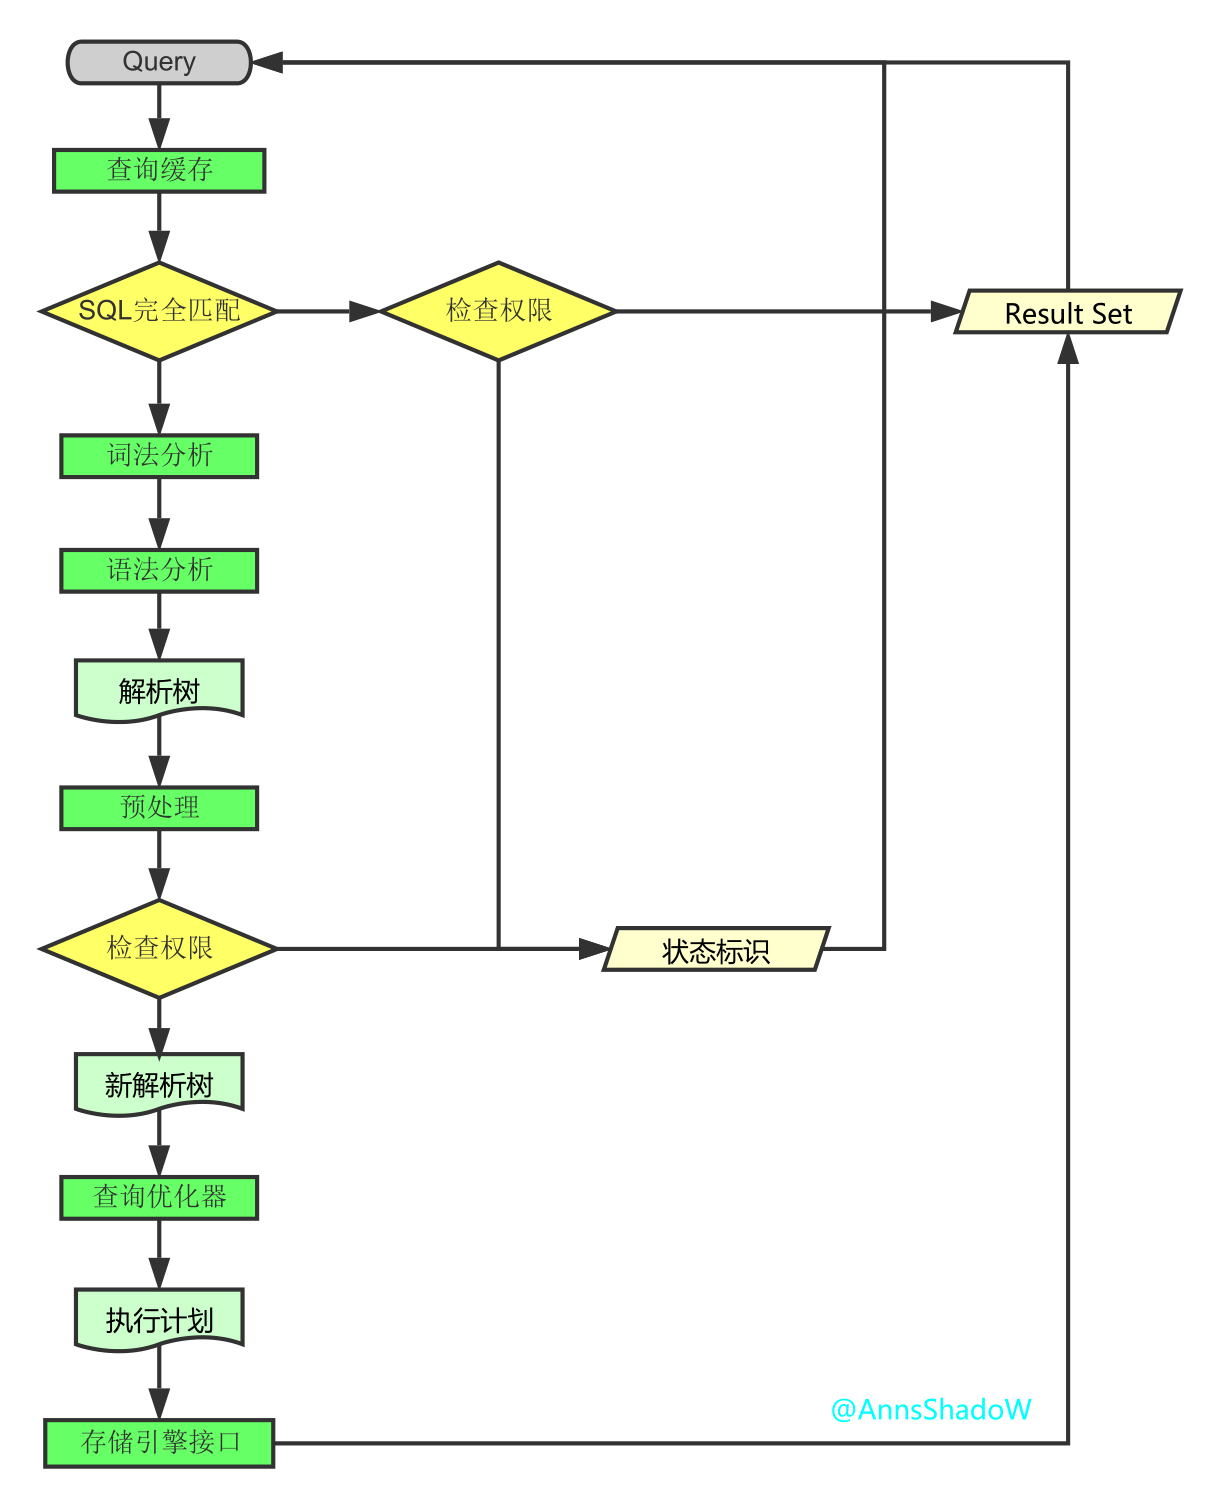
\includegraphics[width=17cm,height=13cm]{mysqlProcess}
				\caption{查询执行流程}
			\end{figure}
			
	\section{基本查询语句}
		\subsection{条件查询}
				\begin{table}[H]
					\centering
					\caption{查询符号}
					\begin{longtable}{c|m{10cm}}
						\hline
						运算符   &   功能说明\\
						\hline
						\verb|=| &  等于 \\
						\verb|!=| & 不等于 \\
						\verb|between ... and ..| & 等同于 \verb|>= ... and <= ...| \\
						\verb|is null| & 为\verb|null(is not null 不为空)| \\
						\verb|and| & 并且 \\
						\verb|or| & 或者\\
						\verb|in| & 包含,相当于多个\verb|or|,(not in 不在这个范围内)\\
						\verb|not| & 取非\\
						\verb|like| & 为模糊查询,支持\verb|%|或\verb|_|匹配,其中\verb|%|匹配任意个字符,\verb|_|只匹配一个字符\\
						\hline	
					\end{longtable}
				\end{table}
				
		\verb|example ->| 
			\begin{lstlisting}
// 执行顺序
	select  // 3
		xx, xx2, xx3
	 from   // 1
		XX
	 where  // 2
		 xx = xx;
		 
// in 示例	查找job是什么的,不是什么的	 
	select 
		ename,job
	from
		emp
	where
		job in('MANAGER','SALESMAN');
		
	select 
		ename,job
	from
		emp
	where
		job not in('MANAGER','SALESMAN');

// like 示例, 查找以S 开头的名字
	select 
		ename
	from 
		emp
	where
		ename like 'S%'	
			\end{lstlisting}
			
		\subsection{排序}
			\verb|order  by|
		
			\begin{lstlisting}
// order  示例 默认升序,(desc 降序)
select 
	ename,salary
from
	emp
order by
	salary

// 按照第几个字段排序	
select 
	ename,salary // 1,2 字段
from
	emp
order by
	2  // 第2个字段
	
// 多个字段排序, ename 升序,salary 降序,使用逗号分割
select 
	ename,salary
from
	emp
order by
	salary desc, ename
			\end{lstlisting}
		
		
		\subsection{数据处理函数(单行)}处理单行后结束
			\begin{itemize}[itemindent = 2em]
				\item \verb|lower| :转换小写
				\item \verb|upper| :转换大写
				\item \verb|substr| :取子串(被截取的串,起始位置,截取长度)
				\item \verb|length| :取长度
				\item \verb|trim| :去空格
				\item \verb|round| :四舍五入
				\item \verb|rand()| :生成随机数
				\item \verb|ifnull(xx, num)|: 可以将\verb|null| 值转换成一个具体值
			\end{itemize}
		
		
		\subsection{分组函数、聚合函数(多行)}
		
			处理多行后结束,自动忽略空值
			
			\textbf{先分组,然后再执行分组函数}, 而where在分组函数之前执行,所以不能
			
			\verb|where| 中不能出现分组函数
			
			\begin{itemize}[itemindent = 2em]
				\item \verb|count |:取得记录数
				\item \verb|sum |:求和
				\item \verb|avg |:求平均
				\item \verb|max |:取最大值
				\item \verb|min |:取最小值
			\end{itemize}
			
			\verb|distinct 去重关键字 -> select distinct job from emp;|  只能出现在所有\textbf{字段}的最前面
			
			\verb|select count(distinct job) from emp;|
			
	\section{分组查询}
			\subparagraph{group by}: \textbf{通过哪个或哪些字段进行分组},使用后select 后只能跟参与分组的字段和分组函数。
			
				\verb|example->| 找出每个工作岗位的最高薪水【先按照工作岗位分组,使用max 函数求每一组的最高工资】
				
					\begin{lstlisting}
// 先按照job 分组,然后对每一组使用max(salary) 求最大值。					
	select 			//3
		max(salary)
	from			//2
		emp;
	group by		//1
		job;	
		
// 结合where 限定分组前条件,即分组前过滤
	select
		job, max(sal)
	from 
		emp
	where 
		job != 'MANAGER'
	group by
		job;
	
					\end{lstlisting}
			
				\verb|example->| 找出每个工作岗位的平均薪水,要求显示平均薪水大于1500
				 where  处理不了
				
			\subparagraph{having} 与where 都是为了完成数据的过滤, \verb|where| 和 \verb|having| 后面都是添加过滤条件,\textbf{where是 在group by 之前执行}, \textbf{而having 是在group  by  后执行}。
			
				\begin{lstlisting}
//上例子解法
select 
	job,avg(sal)
from 
	emp
group by
	job
having 
	avg(sal) >  1500;
 
				\end{lstlisting}
			
			
			\subsection{查询语句总结}
			
				\subparagraph{关键字顺序不能变}:
				
					\begin{lstlisting}
	select 
		...
	from
		...
	where
		...
	group by
		...
	having
		...
	order by
		...
					\end{lstlisting}
			
				\subparagraph{执行顺序}:
					\begin{enumerate}[itemindent = 2em]
						\item \verb|from| 从某张表中检索数据
						\item \verb|where| 经过某条件进行过滤
						\item \verb|group by| 然后分组
						\item \verb|having| 分组之后不满意再过滤
						\item \verb|select| 查询出来
						\item \verb|order by| 排序输出
					\end{enumerate}
		
\section{连接查询}
	查询的时候\textbf{只从一张表检索数据}称为单表查询
	
	在实际的开发中,数据并不是存储在一张表中的,是同时存储在多张表中,这些表和表之间存在关系,我们在检索的时候通常需要将多长表联合起来取得有效数据,这种\textbf{多表查询}被\textbf{称为连接查询}或者叫做跨表查询。
	
	连接查询根据连接方式可以分为如下方式:
		\begin{itemize}[itemindent = 2em]
			\item  内连接
				\begin{itemize}[itemindent = 3em]
					\item 等值连接
					\item 非等值连接
					\item 自连接
				\end{itemize}
				
			\item  外连接
				\begin{itemize}[itemindent = 3em]
					\item 左外连接
					\item 右外连接
				\end{itemize}
				
			\item  全连接【几乎不用】
		\end{itemize}
		
		\begin{figure}[H]
			\centering
			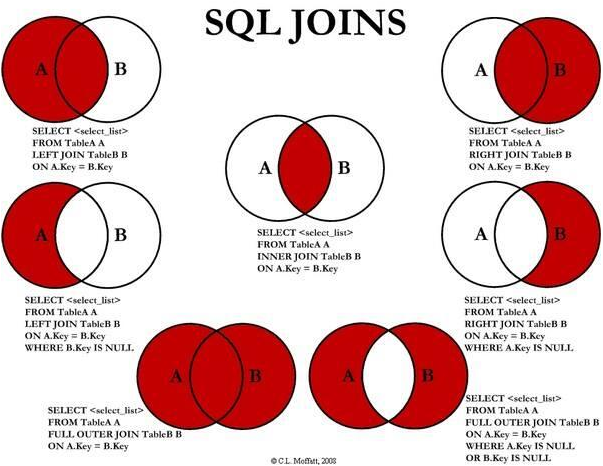
\includegraphics[scale=.76]{joins}
			\caption{SQL Joins}
		\end{figure}
		
	\subsection{内连接}		
			查找两张表匹配的数据。
			
			A表和B表能够完全匹配的记录查询出来,被称为内连接。
			\begin{figure}[H]
				\centering
				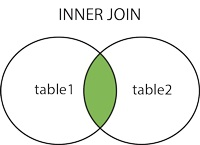
\includegraphics[scale=1]{innoJoin}
				\caption{内连接}
			\end{figure}
			
			\subparagraph{别名的使用,内连接的等值连接} 在进行多表连接查询的时候,尽量给表起别名,这样效率高,可读性高
				\begin{lstlisting}
// 将表emp 用别名 e表示..	

// 查询员工名与其对应的部门名
	select	
		e.ename, d.dname
	from 
		emp e, dept d;
	where 
		e.depno = d.depno
		
// SQL99 语法,使得表连接独立出来了,结构更清晰
	select 
		e.ename, d.dname
	from 
		emp e
	join	  // 内连接的inner 可以省略 
	    dept d
	on 
		e.depno = d.depno;
					\end{lstlisting}
					
				\subparagraph{内连接的非等值连接} 范围
					\begin{lstlisting}
// 找出员工名, 薪水,与其的薪水等级
	select 	
		e.name, e.sal, s.grade
	from
		emp e
	join 
		salgrade s
	on e.sal >= s.lower and e.sal <= s.higher;  // 可以使用between and 替代
					\end{lstlisting}
				 
				
				\subparagraph{内连接的自连接} 自己与自己连接,将自己视为两张表
					\begin{lstlisting}
//  找出每一个员工的上级领导,要求显示员工名以及对应的领导名
	表结构:
	empno ename mgr
	7369  SMITH 7123

// 要点:将自己视为两张表
	select
		a.ename empname, b.ename leaderName
	from 
		emp a
	join
		emp b
	on 
		a.mgr = b.empno;
					\end{lstlisting}	
				
	\subsection{外连接}

		A表和B表能够匹配的记录查询出来之外,\textbf{将其中一张表的记录}\textit{\underline{完全无条件}}的\textbf{完全查询出来},\textit{对方表没有匹配的记录,会自动模拟出NULL与之匹配}。
		
		$$\verb|外连接查询的结构条数| >= \verb|内连接的查询结果数量|$$
		
		可以添加除了内连接外的其他数据。
		\begin{figure}[H]
			\centering
			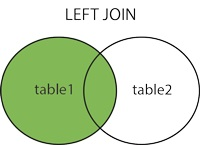
\includegraphics[scale=1]{leftjoin}
			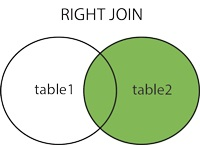
\includegraphics[scale=1]{rightjoin}
			\caption{外连接(左右)}
		\end{figure}
		
		
		\verb|example ->|找出每一个员工对应的部门名称,并且显示所有部门名称,注意部门可能没有员工。
		
				
		\subparagraph{左外连接}
			\verb|select e.ename, d.dname  from dept d left join emp e on e.deptno = d.deptno;|
		
		\subparagraph{右外连接}
			\verb|select e.ename, d.dname  from emp e right join dept d on e.deptno = d.deptno;|// outer  省略
				
		
		\subparagraph{总结}
			\textbf{希望将哪边表的数据完全显示出来},\verb| join| 的前边的修饰词 \verb|right left| 可以恰好说明,如上,\textbf{希望将dept表完全显示},那么\verb|先写dept| 的话,那么就在\verb|join 的左边|,就是 \verb|left join|.	
			
	
	\subsection{内连接外连接 原理性能分析}
		\url{https://www.cnblogs.com/cdf-opensource-007/p/6507678.html}
		
		\url{https://www.cnblogs.com/cdf-opensource-007/p/6517627.html}
	
	\section{子查询}
		\url{https://www.cnblogs.com/zhuiluoyu/p/5822481.html}
	
	\section{union}
		UNION 操作符用于合并两个或多个 SELECT 语句的结果集
		
		\begin{lstlisting}
	SELECT column_name(s) FROM table_name1 // 如只有 1
	UNION
	SELECT column_name(s) FROM table_name2 // 如只有 2
	
	// 则结果为
	1
	2
		\end{lstlisting}	
		
		示例:\url{http://www.w3school.com.cn/sql/sql_union.asp}
			
	\section{limit}		
		用来获取一张表中的\textbf{某部分数据},只在MySQL数据特有的。
		\begin{lstlisting}
	// 找到员工表中前5条记录
	select ename 
	from emp 
	limit 5; //从下标0开始
	
	select ename
	from emp
	limit 0,5;// 从0下标开始,查找前5条
	
	// 找到工资在3到9名的员工
	select salary 
	form emp
	order by salary desc 
	limit 2,7;// 第三个的下标为2,一共7条
		\end{lstlisting}
	
	
	\section{执行顺序}
		\begin{figure}[H]
			\centering
			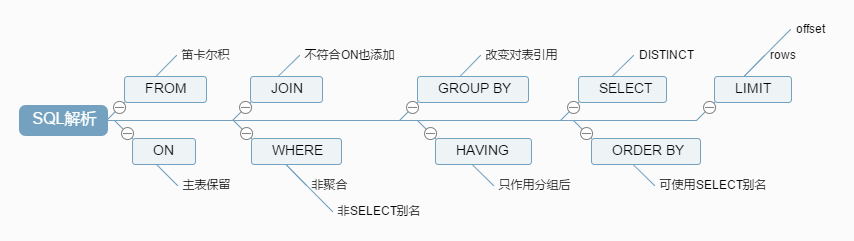
\includegraphics[scale=.6]{sqlProcess}
			\caption{SQL 解析顺序}
		\end{figure}
		
		\begin{lstlisting}
	FROM <left_table>
	ON <join_condition>
	<join_type> JOIN <right_table>
	WHERE <where_condition>
	GROUP BY <group_by_list>
	HAVING <having_condition>
	SELECT 
	DISTINCT <select_list>
	ORDER BY <order_by_condition>
	LIMIT <limit_number>
		\end{lstlisting}
		
	\section{执行过程}
		\url{https://www.cnblogs.com/cdf-opensource-007/p/6502556.html}
		
		\begin{enumerate}
			\item \textbf{加载数据表至内存}:一条查询的sql语句\textbf{先执行的是} \verb|FROM student| 负责\textbf{把数据库的表文件加载到内存中去}。(mysql数据库在计算机上也是一个进程,cpu会给该进程分配一块内存空间)
			\item \textbf{条件过滤}:\verb|WHERE grade < 60|,会把所示\textit{表中的数据进行过滤},\textbf{取出符合条件的记录行,生成一张临时表}
			\item \textbf{分组}:\verb|GROUP BY `name`|会把临时表在内存中切分成若干临时表。
			\item \textbf{选择}:\textbf{SELECT 的执行读取规则}分为sql语句中有无GROUP BY两种情况。
				\begin{itemize}
					\item 当没有GROUP BY时,SELECT 会根据后面的字段名称对内存中的一张临时表整列读取。
					\item 当查询sql中有GROUP BY时,会对内存中的若干临时表分别执行SELECT,而且只取各临时表中的第一条记录,然后再形成新的临时表。这就决定了查询sql使用GROUP BY的场景下,SELECT后面跟的一般是参与分组的字段和聚合函数,否则查询出的数据要是情况而定。另外聚合函数中的字段可以是表中的任意字段,需要注意的是聚合函数会自动忽略空值。
				\end{itemize}
			\item \textbf{对分组后的数据再次过滤}:\verb|HAVING num >= 2|对上图所示临时表中的数据再次过滤,与\verb|WHERE语句|不同的是\verb|HAVING| 用在\verb|GROUP BY|之后,\verb|WHERE|是对\verb|FROM student|从数据库表文件加载到内存中的原生数据过滤,而\verb|HAVING |是对\verb|SELECT |语句执行之后的临时表中的数据过滤。
			\item \textbf{对以上的临时表进行排序}:\verb@ORDER BY xx DESC|ASC@
		\end{enumerate}
		
	
	
	\section{视图 View}
		一种虚拟的表,将查询封装到该视图中。
		
		视图可以包含表的全部或者部分记录,也可以由一个表或者多个表来创建。使用视图就可以不用看到数据表中的所有数据,而是只想得到所需的数据。当我们创建一个视图的时候,\textbf{实际上是}\textit{在数据库里执行了}\verb|SELECT|\textit{语句},\verb|SELECT|\textit{语句包含了字段名称、函数、运算符,来给用户显示数据}。
		
		视图在外观上和表很相似,但是它不需要实际上的物理存储,\textbf{数据还是存储在原来的表里}。\textit{在数据库中,只存放了视图的定义}。
		
		视图的\textbf{使用方式与表的使用方式一致}。
		
		基于视图可以创建视图。
		
		视图\textbf{增加了数据的安全性和逻辑独立性},数据库的设计和结构不会受到视图中的函数、where 或 join 语句的影响。视图可以只展现数据表的一部分数据,对于我们不希望让用户看到全部数据,只希望用户看到部分数据的时候,可以选择使用视图。
		
		更新视图可以更新真实表。
		
		\subsection{创建}
			\begin{lstlisting}
	CREATE [ALGORITHM = {MERGE  | TEMPTABLE | UNDEFINED}]  VIEW 视图名称[(column_list)] AS SELECT 语句  WITH  [CASCADED|LOCAL] CHECK OPTION
	
	create view employee_view as SELECT * from employee;			
			\end{lstlisting}
			首先,第一个中括号里代表的就是创建视图是的算法属性,它允许我们控制\verb|mysql|在创建视图时使用的机制,并且\verb|mysql|提供了三种算法:\verb|MERGE|,\verb|TEMPTABLE| 和 \verb|UNDEFINED|。	
			
			
			\begin{itemize}
				\item \textbf{使用MERGE算法},mysql首先\textbf{将输入查询与定义视图的select语句组合成单个查询。 然后mysql执行组合查询返回结果集}。 \textit{如果}select语句\textbf{包含集合函数}(如min,max,sum,count,avg等)\textbf{或}distinct,group by,havaing,limit,union,union all,\textbf{子查询},\textbf{则不允许使用MERGE算法}。 \textit{如果}select\textbf{语句无引用表},\textbf{则也不允许使用MERGE算法}。 如果不允许MERGE算法,mysql将算法更改为UNDEFINED。我们要注意,将视图定义中的输入查询和查询组合成一个查询称为视图分辨率。
				
				\item \textbf{使用TEMPTABLE算法},mysql首先\textbf{根据定义视图的SELECT语句创建一个临时表,然后针对该临时表执行输入查询}。因为mysql必须创建临时表来存储结果集并将数据从基表移动到临时表,所以TEMPTABLE算法的效率比MERGE算法效率低。 另外,\textbf{使用TEMPTABLE算法的视图是不可更新的}。
				
				\item \textit{当我们创建视图而不指定显式算法时},\textbf{UNDEFINED是默认算法}。 UNDEFINED算法使mysql可以选择使用MERGE或TEMPTABLE算法。mysql优先使用MERGE算法,因为MERGE算法效率更高。
			\end{itemize}
			
			\begin{itemize}
				\item \verb|CASCADED| 默认值,表示更新视图的时候,要满足视图和表的相关条件
				\item \verb|LOCAL|:表示更新视图的时候,要满足该视图定义的一个条件即可
			\end{itemize}
			
			\verb|with check option|:对视图进行更新操作的时,需要检查更新后的值是否还是满足视图公式定义的条件。通俗点,就是所更新的结果是否还会在视图中存在。如果更新后的值不在视图范围内,就不允许更新如果创建视图的时候,没有加上\verb|with check option|,更新视图中的某项数据的话,mysql并不会进行有效性检查。删掉了就删掉了。在视图中将看不到了。所以使用WHIT [CASCADED|LOCAL] CHECK OPTION选项可以保证数据的安全性
			
		\subsection{查看视图数据}
			\begin{lstlisting}
	SELECT * FROM employee_view;		
			\end{lstlisting}		
		
		\subsection{查看视图}	
			\begin{lstlisting}
	show CREATE view employee_view;		
			\end{lstlisting}		
		
		\subsection{删除视图}
			\begin{lstlisting}
	drop view employee_view		
			\end{lstlisting}		
		
		\subsection{修改视图}
			\begin{lstlisting}
	create or replace view employee_view as select eid,ename,salary FROM employee;
	
	alter view employee_view as SELECT * FROM employee;		
			\end{lstlisting}		
		
		\subsection{修改视图中的数据}
			\begin{lstlisting}
	UPDATE employee_view set ename='小红' WHERE ename='小个';		
			\end{lstlisting}	
		
\chapter{增、删、改}
	\section{表、(with约束)}
		\subsection{create table tableName(columName type(length) [constraints]);}
			\begin{lstlisting}
	create table tableName(
		columnName dataType(length) constraints,
		...
	);
	set character_set_result = 'gbk';
	
	drop table tableName;
	drop table if exist tableName; //MySql 特色
	
	create table tableName as select * from existTableName; // 根据已创建的表创建新表
			\end{lstlisting}
		
		\subsection{数据类型}
			\begin{itemize}
				\item \verb|VARCHAR |可变长度字符串
				\item \verb|CHAR |定长字符串
				\item \verb|INT、BIGINT、FLOAT、DOUBLE | 基础数据类型
				\item \verb|DATE | 日期类型
				\item \verb|BLOB | 2进制大对象->图片
				\item \verb|CLOB | 字符大对象->比较大的字符串
			\end{itemize}
			
	\section{表结构}	
		\subsection{alter table tableName add newColumeName type(length);}
		
		\subsection{alter table tableName modify column newType(lenght);}
		
		\subsection{alter table tableName drop column;}
	
	
		
	\section{数据}
		\subsection{insert into tableName(column,..) values (value1,...);}
		
		\subsection{update tableName set columnName=newValue,... where xx;}
			当不指定条件时,将全表的该字段全部更新。
		
		\subsection{delete from tableName where xx;}
	
	
		
	\section{约束}
		\subsection{非空约束 not null}
			不能为空
			
		\subsection{唯一性约束 unique}
			不能重复但是可以为NULL,该字段值具有唯一性
			
			\paragraph{列级约束}
				\begin{lstlisting}
	create table tb(
	..,
	column varchar(32) unique,
	..);
				\end{lstlisting}
				
			\paragraph{表级约束}
				\begin{lstlisting}
	create table tb(
		...,
		column varchar(32),
		...,
		constraint consName unique(column1,...)
	);
				\end{lstlisting}
			
			当使用表级约束时,表示\textbf{多个字段联合}起来后唯一即可。而表级约束可以有名称是为了以后方便删除该约束。
			
		\subsection{主键约束 primary key}
			此列必须是\textbf{唯一并且非空}
			
			每个表都应该有一个主键,并且每个表只能有一个主键。但是注意,并不是说该主键只能在一列上作用,它具有表级约束的联合约束特性。
			\begin{lstlisting}
CREATE TABLE Persons
(
	P_Id int NOT NULL,
	LastName varchar(255) NOT NULL,
	FirstName varchar(255),
	Address varchar(255),
	City varchar(255),
	CONSTRAINT pk_PersonID PRIMARY KEY (P_Id,LastName)
)

			\end{lstlisting}
			在上面的实例中,只有一个主键 \verb|PRIMARY KEY(pk_PersonID),|然而,\verb|pk_PersonID| 的值是由两个列\verb|P_Id 和 LastName)|组成的。
			
		\subsection{外键约束 foreign key}
			\textbf{一个表中的} \verb|FOREIGN KEY| \textbf{指向另一个表中的} \verb|PRIMARY KEY|.
			
			\textbf{“Persons” 表}中的 \verb|“P_Id”| 列\textbf{是 “Persons” 表}中的 \verb|PRIMARY KEY|。
			
			\textbf{“Orders” 表}中的 \verb|“P_Id” |列\textbf{是 “Orders” 表}中的 \verb|FOREIGN KEY|。
			
			\verb|FOREIGN KEY| 约束用于\textbf{预防破坏表之间连接的行为}。
			
			\verb|FOREIGN KEY| 约束也能\textbf{防止非法数据插入外键列},\textit{因为它必须是它指向的那个表中的值之一}。
			
			\begin{lstlisting}
CREATE TABLE Orders
(
	O_Id int NOT NULL,
	OrderNo int NOT NULL,
	P_Id int,
	PRIMARY KEY (O_Id),
	FOREIGN KEY (P_Id) REFERENCES Persons(P_Id)
)
			\end{lstlisting}
	
	
	
	\section{触发器 Trigger}
		触发器\textbf{是与表有关的数据库对象},在满足定义条件时触发,并执行触发器中定义的语句集合。触发器的这种特性可以协助应用在数据库端确保数据的完整性。
	
		\begin{figure}[H]
			\centering
			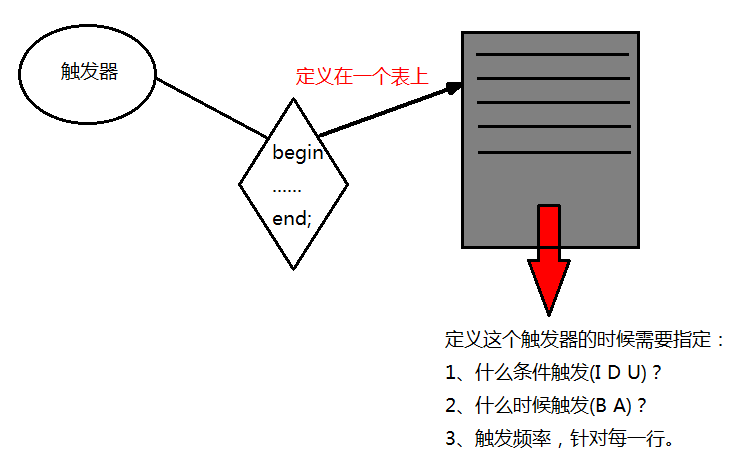
\includegraphics[width=15cm,height=5cm]{trigger}
			\caption{触发器结构演示}
		\end{figure}
		
		\subparagraph{特性}
			\begin{itemize}
				\item 有\verb|begin end|体,\verb|begin end|;之间的语句可以写的简单或者复杂
				\item \textbf{什么条件}会触发:Insert、Update、Delete
				\item \textbf{什么时候}触发:在增删改\textbf{前或者}后
				\item 触发频率:\textbf{针对每一行执行}
				\item 触发器定义在表上,附着在表上。
				\item \textbf{cannot} associate a \textbf{Trigger} with a \textbf{TEMPORARY table} or a \textbf{View}.
				\item 触发器是针对每一行的;对增删改非常频繁的表上切记不要使用触发器,因为它会非常消耗资源。 
			\end{itemize}
		
		
		\subsection{创建触发器}
			\begin{lstlisting}
CREATE
    [DEFINER = { user | CURRENT_USER }]
TRIGGER trigger_name
trigger_time trigger_event
ON tbl_name FOR EACH ROW
  [trigger_order]
trigger_body

trigger_time: { BEFORE | AFTER }

trigger_event: { INSERT | UPDATE | DELETE }

trigger_order: { FOLLOWS | PRECEDES } other_trigger_name			
			\end{lstlisting}
		
			 \verb|FOR EACH ROW| 表示任何一条记录上的操作满足触发事件都会触发该触发器,也就是说触发器的\textbf{触发频率是针对每一行数据触发一次}。

			
			\paragraph{创建只有一个执行语句的触发器}
				\begin{lstlisting}
CREATE TRIGGER 触发器名 BEFORE|AFTER 触发事件 ON 表名 FOR EACH ROW 执行语句;				
				\end{lstlisting}
			
			\paragraph{创建有多个执行语句的触发器}
				\begin{lstlisting}
CREATE TRIGGER 触发器名 BEFORE|AFTER 触发事件
ON 表名 FOR EACH ROW
BEGIN
        执行语句列表
END;				
				\end{lstlisting}
		
		
		\subsection{查看触发器}	
			\begin{itemize}
				\item \verb|SHOW TRIGGERS;|
				\item \verb|SELECT * FROM information_schema.triggers;|
			\end{itemize}
			
			
		\subsection{删除触发器}
			\begin{lstlisting}
DROP TRIGGER [IF EXISTS] [schema_name.]trigger_name
			\end{lstlisting}


\chapter{存储过程}
	\url{http://www.runoob.com/w3cnote/mysql-stored-procedure.html}
	
	存储过程就\textbf{类似于脚本}。
	
	存储过程是\textbf{为了完成特定功能的SQL语句集},经编译创建并保存在数据库中,用户可通过指定存储过程的名字并给定参数(需要时)来调用执行。
	
	\section{存储过程的创建和调用}
		\begin{lstlisting}
CREATE
    [DEFINER = { user | CURRENT_USER }]
 PROCEDURE sp_name ([proc_parameter[,...]])
    [characteristic ...] routine_body
 
proc_parameter:
    [ IN | OUT | INOUT ] param_name type
 
characteristic:
    COMMENT 'string'
  | LANGUAGE SQL
  | [NOT] DETERMINISTIC
  | { CONTAINS SQL | NO SQL | READS SQL DATA | MODIFIES SQL DATA }
  | SQL SECURITY { DEFINER | INVOKER }
 
routine_body:
  Valid SQL routine statement
 
[begin_label:] BEGIN
  [statement_list]
    ……
END [end_label]		
		\end{lstlisting}
	
	
		\subsection{声明语句结束符}
			\begin{lstlisting}
DELIMITER $$
或
DELIMITER //			
			\end{lstlisting}
		
		\subsection{声明存储过程}
			\begin{lstlisting}
CREATE PROCEDURE demo_in_parameter(IN p_in int)       			
			\end{lstlisting}		
		
		\subsection{存储过程开始和结束符号}
			\begin{lstlisting}
BEGIN .... END  			
			\end{lstlisting}
		
		\subsection{变量赋值}
			\begin{lstlisting}
SET @p_in=1  			
			\end{lstlisting}
		
		\subsection{变量定义}		
			\begin{lstlisting}
DECLARE l_int int unsigned default 4000000; 			
			\end{lstlisting}
			
		\subsection{创建存储过程、存储函数名(参数)}
			\begin{lstlisting}
create procedure 存储过程名(参数)			
			\end{lstlisting}		
		
		\subsection{存储过程体}
			\begin{lstlisting}
create function 存储函数名(参数)			
			\end{lstlisting}			
		
		\subsection{实例}
			\begin{lstlisting}
mysql> delimiter $$  #将语句的结束符号从分号;临时改为两个$$(可以是自定义)
mysql> CREATE PROCEDURE delete_matches(IN p_playerno INTEGER)
    -> BEGIN
    ->   DELETE FROM MATCHES
    ->    WHERE playerno = p_playerno;
    -> END$$
Query OK, 0 rows affected (0.01 sec)
 
mysql> delimiter;  #将语句的结束符号恢复为分号    			
			\end{lstlisting}
			
			\begin{lstlisting}
mysql> select * from MATCHES;
+---------+--------+----------+-----+------+
| MATCHNO | TEAMNO | PLAYERNO | WON | LOST |
+---------+--------+----------+-----+------+
|       1 |      1 |        6 |   3 |    1 |
|       7 |      1 |       57 |   3 |    0 |
|       8 |      1 |        8 |   0 |    3 |
|       9 |      2 |       27 |   3 |    2 |
|      11 |      2 |      112 |   2 |    3 |
+---------+--------+----------+-----+------+
5 rows in set (0.00 sec)
 
mysql> call delete_matches(57);
Query OK, 1 row affected (0.03 sec)
 
mysql> select * from MATCHES;
+---------+--------+----------+-----+------+
| MATCHNO | TEAMNO | PLAYERNO | WON | LOST |
+---------+--------+----------+-----+------+
|       1 |      1 |        6 |   3 |    1 |
|       8 |      1 |        8 |   0 |    3 |
|       9 |      2 |       27 |   3 |    2 |
|      11 |      2 |      112 |   2 |    3 |
+---------+--------+----------+-----+------+
4 rows in set (0.00 sec)			
			\end{lstlisting}

	\section{存储过程的参数}
	
	
	
	\section{存储过程的变量}


\chapter{游标}
	有数据缓冲的思想:游标的设计\textbf{是一种数据缓冲区的思想,用来存放SQL语句执行的结果}。 
	
	游标是\textit{在先从数据表中检索出数据之后才能继续灵活操作的技术}。 类似于指针:游标类似于指向数据结构堆栈中的指针,用来pop出所指向的数据,并且只能每次取一个。
	
	\section{特点}
		\begin{itemize}
			\item 游标是\textbf{针对行操作的},所以对从数据库中select查询得到的每一行可以进行分开的独立的相同或不同的操作,是一种分离的思想。
			\item 在数据量大的情况下,是不适用的,速度过慢。这里有个比喻就是:当你去ATM存钱是希望一次性存完呢,还是100一张一张的存,这里的100一张一张存就是游标针对行的操作。 数据库大部分是面对集合的,业务会比较复杂,而游标使用\textbf{会有死锁},影响其他的业务操作,不可取。 当数据量大时,使用游标会造成\textbf{内存不足}现象。
		\end{itemize}
	
	\section{创建与使用}
		\subsection{定义游标}
			\begin{lstlisting}
DECLARE <游标名> CURSOR FOR select语句;	

DECLARE mycursor CURSOR FOR select * from shops_info;	
			\end{lstlisting}
		
		\subsection{打开游标}
			\begin{lstlisting}	
open <游标名>			
			\end{lstlisting}
		
		\subsection{使用游标}
			使用游标需要用关键字fetch来取出数据,然后取出的数据需要有存放的地方,我们需要用declare声明变量存放列的数据其语法格式为:
			\begin{lstlisting}
declare 变量1 数据类型(与列值的数据类型相同)
declare 变量2 数据类型(与列值的数据类型相同)
declare 变量3 数据类型(与列值的数据类型相同)
FETCH [NEXT | PRIOR | FIRST | LAST] FROM <游标名> [ INTO 变量名1,变量名2,变量名3[,…] ]			
			\end{lstlisting}
			
			\begin{lstlisting}
-- 声明四个变量
  declare id varchar(20); 
  declare pname varchar(20); 
  declare pprice varchar(20);
  declare pdescription varchar(20);
 
-- 1、定义一个游标mycursor
  declare mycursor cursor for
	select *from shops_info;
-- 2、打开游标
  open mycursor;
-- 3、使用游标获取列数据放入变量中
  fetch  next from mycursor into id,pname,pprice,pdescription; 			
			\end{lstlisting}
			
		\subsection{关闭游标}
			\begin{lstlisting}
close mycursor;			
			\end{lstlisting}
		
		
		\subsection{释放游标}
			\begin{lstlisting}
deallocate mycursor;			
			\end{lstlisting}
		
		
	\section{实例}
		\url{https://www.cnblogs.com/mqxs/p/6018766.html}
		
		\url{https://www.cnblogs.com/progor/p/8875100.html}
		
		\subsection{普通游标}
			\begin{lstlisting}
drop procedure if exists cursor_test;
delimiter //
create procedure cursor_test()
begin
    -- 声明与列的类型相同的四个变量
    declare id varchar(20); 
    declare pname varchar(20); 
    declare pprice varchar(20);
    declare pdescription varchar(20);
 
-- 1、定义一个游标mycursor
    declare mycursor cursor for
   	select *from shops_info;
-- 2、打开游标
    open mycursor;
-- 3、使用游标获取列的值
    fetch  next from mycursor into id,pname,pprice,pdescription; 
-- 4、显示结果
    select id,pname,pprice,pdescription;
-- 5、关闭游标
    close mycursor;
end;
//
delimiter ;
call cursor_test();		
			\end{lstlisting}
		
			当然可以使用循环,while 循环定义如下:
			\begin{lstlisting}
WHILE expression DO
    Statements;
END WHILE
//实例
DECLARE num INT;
DECLARE my_string  VARCHAR(255);
SET num =1;
SET str ='';
  WHILE num  < span>10DO
SET  my_string =CONCAT(my_string,num,',');
SET  num = num +1;
END WHILE;		
			\end{lstlisting}
	
		\subsection{循环游标}	
			\begin{lstlisting}
create procedure p3()
begin
    declare id int;
    declare name varchar(15);
    declare flag int default 0;
    -- 声明游标
    declare mc cursor for select * from class;
    declare continue handler for not found set flag = 1;
    -- 打开游标
    open mc;
    -- 获取结果
    l2:loop 
    
    fetch mc into id,name;
    if flag=1 then -- 当无法fetch会触发handler continue
        leave l2;
    end if;
    -- 这里是为了显示获取结果
    insert into class2 values(id,name);
    -- 关闭游标
    end loop;
    close mc;
    
end;

call p3();-- 不报错
select * from class2;	
			\end{lstlisting}
			
	
\chapter{索引}
	\section{简介}
		索引用于快速找出在某个列中有一特定值的行,不使用索引,MySQL必须从第一条记录开始读完整个表,直到找出相关的行,表越大,查询数据所花费的时间就越多,如果表中查询的列有一个索引,MySQL能够快速到达一个位置去搜索数据文件,而不必查看所有数据,那么将会节省很大一部分时间。

		\textbf{例如}:\textit{有一张person表,其中有2W条记录,记录着2W个人的信息。有一个Phone的字段记录每个人的电话号码,现在想要查询出电话号码为xxxx的人的信息}。
			\begin{itemize}
				\item \textbf{如果没有索引},那么将从表中第一条记录一条条往下\textbf{遍历},直到找到该条信息为止。
				\item \textbf{如果有了索引},那么会将\textbf{该Phone字段},\textbf{通过一定的方法进行存储},\textit{好让查询该字段上的信息时,能够快速找到对应的数据},而不必在遍历2W条数据了。其中MySQL中的索引的存储类型有两种:\verb|BTREE|、\verb|HASH|。
			\end{itemize}
			
			\begin{figure}[H]
				\centering
				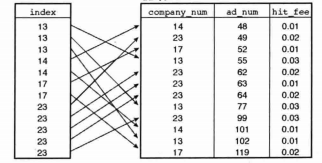
\includegraphics[width=13cm,height=5cm]{index}
				\caption{索引后的表样例}
			\end{figure}
			
			加了索引后,就不用一行行的搜索整个表了,我们可以使用这个索引。假设,我们要找处公司编号为13 的所有行,我们开始扫描索引,便会找到3个属于该公司的值,然后会找到到达公司编号为14的索引值,该值比我们正查找的值要大一点,由于索引值是有序的,因此当我们独到那条14的索引行时,我们便知道无法找到更多与13匹配的内容了,于是可以退出查找过程,当然这个索引的查找方法可以使用BTREE 和 HASH进行优化加速。
			
			
			对于不同的MySQL存储引擎,索引的具体实现细节会有所不同。
			
			对于MyISAM表,\textbf{其数据行保留在数据文件里,而索引值则保留在索引文件里}。一个表可以有多个索引,但它们都存在一个索引文件里。索引文件里的每一个索引都由一组有序的关键字行构成,这个组关键字行主要用于快速访问数据文件。
			
			对于Innodb, 并没有按照上面的方法将行和索引分开放置,尽管它也是把索引值当作是一组有序值。默认情况下,InnoDB 只使用一个表空间,在这个表空间的内部,管理着所有InnoDB 表的数据存储和索引存储。 可以配置InnoDB, 让它创建的每个表都有自己的表空间。但是即使如此,\textbf{给定表的数据和索引也同样保存在同一个表空间文件里}。
			
	
	\section{索引的分类}
		\subparagraph{存储引擎支持类型}
			索引是在存储引擎中实现的,也就是说不同的存储引擎,会使用不同的索引
			\begin{itemize}[itemindent = 2em]
				\item \verb|MyISAM和InnoDB|存储引擎:\textbf{只支持BTREE索引}
				\item \verb|MEMORY/HEAP|存储引擎:\textbf{支持HASH和BTREE索引}
			\end{itemize}
			
		\subparagraph{单列索引}
			一个索引只包含单个列,但一个表中可以有多个单列索引。主要包括以下几种类型:
			\begin{enumerate}[itemindent = 2em]
				\item 普通索引:基本索引类型,没有什么限制,允许在定义索引的列中插入重复值和空值
				\item 唯一索引:索引列中的值必须是唯一的,但是允许为空值
				\item 主键索引:是一种特殊的唯一索引,不允许有空值。
			\end{enumerate}
			
		\subparagraph{组合索引}
			在表中的多个字段组合上创建的索引,\textbf{只有}在查询条件中\textit{使用了}\textbf{这些字段的左边字段时},索引才会被使用,使用组合索引时遵循最\textbf{左前缀集合}。
		
			\textbf{联合索引左侧字段用了范围查询,则其他字段无法用上}。
			
		
		
			
	\section{优点、缺点和使用原则}
		\subparagraph{优点}
			\begin{itemize}[itemindent = 1em]
				\item 所有的MySql\textbf{列类型}(字段类型)\textbf{都可以被索引},也就是\textit{可以给任意字段设置索引}
				\item 大大加快数据的查询速度
			\end{itemize}
			
		\subparagraph{缺点}
			\begin{itemize}[itemindent = 1em]
				\item 创建索引和维护索引要耗费时间,并且随着数据量的增加所耗费的时间也会增加,表的索引越多,需要做出的更改就越多。
				\item 索引也需要占空间
				\item 当对表中的数据进行增加、删除、修改时,索引也需要动态的维护,降低了数据的维护速度,降低了大部分与写入相关的操作的速度。
			\end{itemize}
			
		\subparagraph{使用原则}
			通过上面说的优点和缺点,我们应该可以知道,并不是每个字段度设置索引就好,也不是索引越多越好,而是需要自己合理的使用。
			\begin{itemize}[itemindent = 1em]
				\item \textbf{对经常更新的表}就\textit{避免对其进行过多的索引},对经常用于查询的字段应该创建索引
				\item \textbf{数据量小的表最好不要使用索引},因为由于数据较少,可能查询全部数据花费的时间比遍历索引的时间还要短,索引就可能不会产生优化效果
				\item \textbf{在一同值少的列上(字段上)不要建立索引},比如\textit{在学生表的"性别"字段上只有男,女两个不同值}。相反的,在一个字段上不同值较多可是建立索引
			\end{itemize}
	
	
	
	\section{挑选索引}
		\begin{itemize}
			\item 为用于搜索、排序、或分组 的列创建索引。
			
				最佳索引候选列是那些出现在WHERE 字句中的列、连接子句中的列, 或者出现在 \verb|ORDER BY|、\verb|GROUP BY| 子句中的列。
				而那些出现在\verb|SELECT| 关键字后面的输出列表里的列,则不是很好的索引候选列。
				
			\item 认真考虑数据列的基数-(非重复值的个数)
				
				一列包含的唯一值多,重复值少,索引使用的效果也会更好。
			
			\item 索引短小值
				
				\begin{itemize}
					\item 短小值可以让比较操作更快,从而加快索引查找速度
					\item 短小值可以让索引短小,从而减少对磁盘的查找速度
					\item 键缓存里索引块可以容纳更多的键值
				\end{itemize}
				
				
			\item 索引字符串值的前缀
			
				针对长字符串可以使用其多少前缀作为索引,以加快查找速度。
			
			
			\item 利用最左前缀-(复合索引)
				
				当创建包含n个列的复合索引时,实际上会创建n个列组合起来的一个字符串 的索引key. 所以需要使用\textbf{最左前缀原则},既如果没有包含其前缀的时候,是无法利用索引加速的。
				
				如 创建的复合索引为 \verb|1、2、3|.
				那么索引可以搜索以下几种组合, \verb|123、12、1|, \textit{对于没有包含最左边前缀的那些搜索},如\textit{按照2或3 来搜索},MySQL \textbf{无法使用索引}。
			
			\item 不要建立过多的索引
			
				对表修改后,涉及到索引的更新,涉及越多,这个过程越耗时,并且索引额外需要占用空间,使得文件更快的到达了最大的文件限制。
			
			\item 让参与比较的索引类型保持匹配
			
			\item 利用慢查询日志找出哪些性能低劣的查询
		\end{itemize}
	

	
	\section{使用方法}	
		\subsection{创建表添加索引}
			\subparagraph{创建普通索引}
				\begin{lstlisting}
	// 方式一
	CREATE TABLE book (
	bookid INT NOT NULL,               
	bookname VARCHAR(255) NOT NULL,           
	authors VARCHAR(255) NOT NULL,            
	info VARCHAR(255) NULL,                
	comment VARCHAR(255) NULL,             
	year_publication YEAR NOT NULL,           
	INDEX(year_publication)               
	);
	
	// 方式二
	CREATE TABLE book (
	bookid INT NOT NULL,               
	bookname VARCHAR(255) NOT NULL,           
	authors VARCHAR(255) NOT NULL,            
	info VARCHAR(255) NULL,                
	comment VARCHAR(255) NULL,             
	year_publication YEAR NOT NULL,           
	KEY(year_publication)               
	);                                                
				\end{lstlisting}
			\subparagraph{创建唯一索引}
				\begin{lstlisting}
	CREATE TABLE t1
	(
	id INT NOT NULL,
	name CHAR(30) NOT NULL,
	UNIQUE INDEX UniqIdx(id)
	); 
				\end{lstlisting}
			\subparagraph{创建主键索引}
				\begin{lstlisting}
	CREATE TABLE t2
	(
		id INT NOT NULL,
		name CHAR(10),
		PRIMARY KEY(id)
	);
				\end{lstlisting}
			
			\subparagraph{创建组合索引}
				\begin{lstlisting}
	CREATE TABLE t3
	(
		id INT NOT NULL,
		name CHAR(30) NOT NULL,
		age INT NOT NULL,
		info VARCHAR(255),
		INDEX MultiIdx(id,name,age)
	);
				\end{lstlisting}
				
				\textbf{组合索引就是遵从了最左前缀},\textit{利用索引中最左边的列集来匹配行,这样的列集称为最左前缀},例如,这里由id、name和age3个字段构成的索引,索引行中就按\verb|id/name/age|的顺序存放,\textbf{索引可以索引下面字段组合}\verb|(id,name,age)|、\verb|(id,name)|或者\verb|(id)|。如果要查询的字段不构成索引最左面的前缀,那么就不会是用索引,比如,age或者\verb|(name,age)|组合\textbf{就不会使用索引查询}
				
		
		\subsection{在已经存在的表上创建索引}
		
			\verb@ALTER TABLE 表名 ADD[UNIQUE|FULLTEXT|SPATIAL] [INDEX|KEY] [索引名](字段名)[ASC|DESC]@
			
			\verb@CREATE [UNIQUE|FULLTEXT|SPATIAL] [INDEX|KEY] 索引名称 ON 表名(字段名[length])[ASC|DESC]@
			
			\begin{itemize}
				\item ALTER TABLE book ADD INDEX BkNameIdx(bookname(30));
				\item CREATE INDEX BkBookNameIdx ON book(bookname);
			\end{itemize}
		
		\subsection{删除索引}
			\begin{itemize}
				\item ALTER TABLE 表名 DROP INDEX 索引名;
				\item DROP INDEX 索引名 ON 表名;
			\end{itemize}
		
		\subsection{使用索引要点}
			\begin{itemize}
				\item 索引可以加快对\verb|WHERE| 字句匹配的行进行搜索的速度,或者用于加快对(\verb|JOIN|)与另一个表里的行进行搜素的速度。
				\item 对于使用\verb|MIN()| 或 \verb|MAX()| 函数的查询,MySQL 可以在不用逐行检查的情况下,快速找到索引列里最小值和最大值。
				\item 对于\verb|ORDER BY| 或 \verb|GROUP BY| 子句,经常使用索引来高效的完成分类和分组操作。
				\item 也会通过索引来读取查询所请求的所有信息(\textit{索引列信息})。
			\end{itemize}
					
	
	\section{索引原理}
		\url{https://www.jianshu.com/p/fa8192853184}
	
		\url{http://blog.codinglabs.org/articles/theory-of-mysql-index.html}
	
		\url{https://draveness.me/sql-index-intro}
		
		\subsection{聚簇索引}
			将数据存储与索引放到了一块,找到索引也就找到了数据
			
			
			\paragraph{辅助索引}
			
			
			
			
			
			
		\subsection{非聚簇索引}
			将数据存储于索引分开结构,索引结构的叶子节点指向了数据的对应行,当需要访问数据时(通过索引访问数据),在内存中直接搜索索引,然后通过索引找到磁盘相应数据.
		
		\subsection{B+ 树}
		
		
		
	\section{参考}
		\url{https://www.cnblogs.com/whgk/p/6179612.html}
			
	
	
\chapter{事务}
	\section{概述}
		一般来说,事务是必须满足4个条件(ACID)::原子性(Atomicity,或称不可分割性)、一致性(Consistency)、隔离性(Isolation,又称独立性)、持久性(Durability)。
		
		\begin{itemize}
			\item \textbf{原子性}:\textit{一个事务(transaction)中的所有操作,要么全部完成,要么全部不完成},不会结束在中间某个环节。事务在执行过程中发生错误,会被回滚(Rollback)到事务开始前的状态,就像这个事务从来没有执行过一样。
			\item \textbf{一致性}:在事务开始之前和事务结束以后,数据库的完整性没有被破坏。这表示写入的资料必须完全符合所有的预设规则,这包含资料的精确度、串联性以及后续数据库可以自发性地完成预定的工作。
			\item \textbf{隔离性}:数据库\textit{允许多个并发事务同时对其数据进行读写和修改的能力,隔离性可以防止多个事务并发执行时由于交叉执行而导致数据的不一致}。事务隔离分为不同级别,包括读未提交(Read uncommitted)、读提交(read committed)、可重复读(repeatable read)和串行化(Serializable)。
			\item \textbf{持久性}:事务处理结束后,对数据的修改就是永久的,即便系统故障也不会丢失。
		\end{itemize}
	
	\section{应用}
		用 \verb|BEGIN|, \verb|ROLLBACK|, \verb|COMMIT|来实现.
		
		\verb|BEGIN| \textbf{开始一个事务}
		
		\verb|ROLLBACK| \textbf{事务回滚}
		
		\verb|COMMIT| \textbf{事务确认}
		
		\begin{lstlisting}
mysql> begin;  # 开始事务
Query OK, 0 rows affected (0.00 sec)
 
mysql> insert into runoob_transaction_test value(5);
Query OK, 1 rows affected (0.01 sec)
 
mysql> insert into runoob_transaction_test value(6);
Query OK, 1 rows affected (0.00 sec)
 
mysql> commit; # 提交事务
Query OK, 0 rows affected (0.01 sec)

mysql>  select * from runoob_transaction_test;
+------+
| id   |
+------+
| 5    |
| 6    |
+------+
2 rows in set (0.01 sec)
 
mysql> begin;    # 开始事务
Query OK, 0 rows affected (0.00 sec)
 
mysql>  insert into runoob_transaction_test values(7);
Query OK, 1 rows affected (0.00 sec)
 
mysql> rollback;   # 回滚
Query OK, 0 rows affected (0.00 sec)
 
mysql>   select * from runoob_transaction_test;   # 因为回滚所以数据没有插入
+------+
| id   |
+------+
| 5    |
| 6    |
+------+
2 rows in set (0.01 sec)		
		\end{lstlisting}

\chapter{锁}
	\url{https://www.cnblogs.com/leedaily/p/8378779.html}
	
	\url{https://www.cnblogs.com/chenqionghe/p/4845693.html}

	锁是计算机\textbf{协调多个进程}或纯线程\textbf{并发访问}某一资源的机制。在数据库中,除传统的计算资源(CPU、RAM、I/O)的争用以外,数据也是一种供许多用户共享的资源。\textit{如何保证数据并发访问的一致性、有效性是所在有数据库必须解决的一个问题,锁冲突也是影响数据库并发访问性能的一个重要因素}。从这个角度来说,锁对数据库而言显得尤其重要,也更加复杂。
	
	
	对于数据库,其实就是\textbf{读写锁}的应用与协调。
	
	
	\section{概述}
		  相对其他数据库而言,MySQL的锁机制比较简单,其最显著的特点是\textbf{不同的存储引擎支持不同的锁机制}。MySQL大致可归纳为以下3种锁:
		  
		  \begin{itemize}
			  	\item \textbf{表级锁}:开销小,加锁快;不会出现死锁;锁定粒度大,发生锁冲突的概率最高,并发度最低。
			  	\item \textbf{行级锁}:开销大,加锁慢;会出现死锁;锁定粒度最小,发生锁冲突的概率最低,并发度也最高。
			  	\item \textbf{页面锁}:开销和加锁时间界于表锁和行锁之间;会出现死锁;锁定粒度界于表锁和行锁之间,并发度一般
		  \end{itemize}
	
	
	\section{Mysql 表级锁-锁模式(MyISAM)}
		MySQL表级锁有两种模式:表共享锁(\verb|Table Read Lock|)和表独占写锁(\verb|Table Write Lock|)
	
		\begin{itemize}
			\item 对MyISAM的\verb|读操作|,\textit{不会阻塞其他用户对同一表的读请求,但会阻塞对同一表的写请求};
			\item 对MyISAM的\verb|写操作|,\textit{则会阻塞其他用户对同一表的读和写操作};
			\item MyISAM表的读操作和写操作之间,以及写操作\textbf{之间是串行的}。
		\end{itemize}

		当一个线程\textbf{获得对一个表的写锁后},\textit{只有持有锁线程可以对表进行更新操作}。\textit{其他线程的读、写操作都会等待,直到锁被释放为止}。
		
		
		MyISAM存储引擎的\textbf{读锁阻塞写例子}: 
		一个\verb|session|使用\verb|LOCK TABLE|命令给表\verb|film_text|\textbf{加了读锁},这个\verb|session|可以查询锁定表中的记录,但更新或访问其他表都会提示错误;同时,另外一个\verb|session|可以查询表中的记录,但更新就会出现锁等待。
		
		\begin{figure}[H]
			\centering
			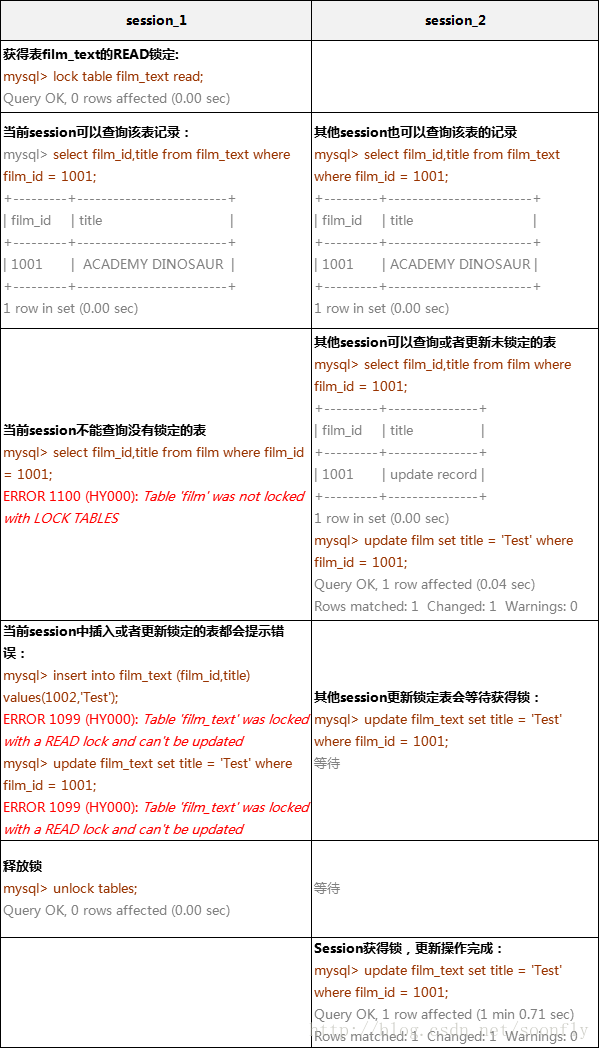
\includegraphics[height=22cm]{lock}
			\caption{锁示例}
		\end{figure}
		
		\subsection{如何加 表锁}
			MyISAM在执行查询语句(\verb|SELECT|)前,\textbf{会自动给涉及的所有表加读锁},在执行更新操作(\verb|UPDATE、DELETE、INSERT|等)前,\textbf{会自动给涉及的表加写锁},\textit{这个过程并不需要用户干预,因此用户一般不需要直接用LOCK TABLE命令给MyISAM表显式加锁}。
			
			在示例中,显式加锁基本上都是为了方便理解而已,并非必须如此。
			
			给\verb|MyISAM|表显示加锁,一般是为了一定程度模拟事务操作,实现对某一时间点多个表的一致性读取。例如,有一个订单表\verb|orders|,其中记录有订单的总金额\verb|total|,同时还有一个订单明细表\verb|order_detail|,其中记录有订单每一产品的金额小计\verb|subtotal|,假设我们需要检查这两个表的金额合计是否相等,可能就需要执行如下两条\verb|SQL|:
			
			\begin{lstlisting}
	SELECT SUM(total) FROM orders;
	SELECT SUM(subtotal) FROM order_detail;
			\end{lstlisting}
			
			这时,如果不先给这两个表加锁,就可能产生错误的结果,因为第一条语句执行过程中,\verb|order_detail|表可能已经发生了改变。因此,正确的方法应该是:
			
			\begin{lstlisting}
	LOCK tables orders read local,order_detail read local;
	SELECT SUM(total) FROM orders;
	SELECT SUM(subtotal) FROM order_detail;
	Unlock tables;	
			\end{lstlisting}
			
			要特别说明以下两点内容。
			
			\begin{itemize}
				\item 上面的例子在\verb|LOCK TABLES|时加了‘\verb|local|’选项,其作用就是在满足\verb|MyISAM|表并发插入条件的情况下,允许其他用户在表尾插入记录
				\item 在用\verb|LOCK TABLES|\textbf{给表显式加表锁是时,必须同时取得所有涉及表的锁},并且MySQL支持锁升级。\textbf{也就是说,在执行LOCK TABLES后,只能访问显式加锁的这些表,不能访问未加锁的表};同时,如果加的是读锁,那么只能执行查询操作,而不能执行更新操作。\textit{其实,在自动加锁的情况下也基本如此},\textbf{MyISAM总是一次获得SQL语句所需要的全部锁}。这也正是MyISAM表不会出现死锁(\verb|Deadlock Free|)的原因
			\end{itemize}
			
			可以通过检查\verb|table_locks_waited| 和 \verb|table_locks_immediate| 状态变量来分析系统上的表锁定争夺
			
			\verb|show status like 'table%';|
			
		\subsection{并发锁}
			上文提到过\verb|MyISAM|表的读和写是串行的,但这是就总体而言的。在一定条件下,\verb|MyISAM|表也支持查询和插入操作的并发进行。 \verb|MyISAM|存储引擎有一个系统变量\verb|concurrent_insert|,专门用以控制其并发插入的行为,其值分别可以为0、1或2。
			
			\begin{itemize}
				\item 当\verb|concurrent_insert|设置为0时,不允许并发插入。
				\item 当\verb|concurrent_insert|设置为1时,如果MyISAM表中没有空洞(即表的中间没有被删除的行),\textbf{MyISAM允许在一个进程读表的同时,另一个进程从表尾插入记录}。这也是MySQL的默认设置。
				\item 当\verb|concurrent_insert|设置为2时,\textbf{无论MyISAM表中有没有空洞,都允许在表尾并发插入记录}。
			\end{itemize}
			
			在下面的例子中,\verb|session_1|获得了一个表的\verb|READ LOCAL|锁,该线程可以对表进行查询操作,但不能对表进行更新操作;其他的线程(\verb|session_2|),虽然不能对表进行删除和更新操作,但却可以对该表进行并发插入操作,这里假设该表中间不存在空洞。
			
			MyISAM存储引擎的读写(INSERT)并发例子:
			\begin{figure}[H]
				\centering
				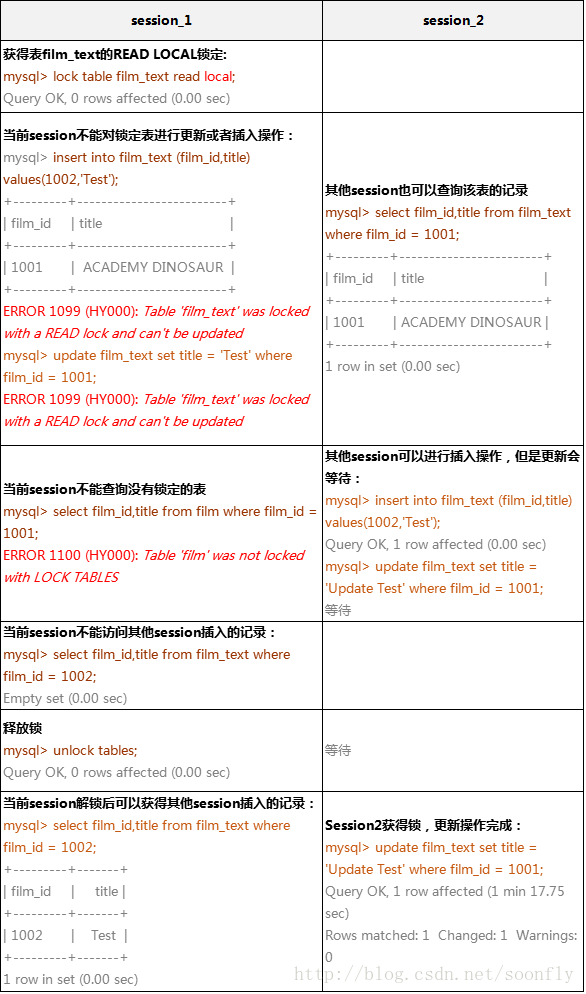
\includegraphics[width=13cm, height=17cm]{lock2}
				\caption{锁示例}
			\end{figure}		
			
			
			可以利用\verb|MyISAM|存储引擎的并发插入特性,来解决应 用中对同一表查询和插入的锁争用。例如,将\verb|concurrent_insert|系统变量设为2,总是允许并发插入;同时,通过定期在系统空闲时段执行 \verb|OPTIMIZE TABLE|语句来整理空间碎片,收回因删除记录而产生的中间空洞
			
		\subsection{锁调度}
			\textit{MyISAM存储引擎的读锁和写锁是互斥的,读写操作是串行的}。那么,一个进程请求某个 MyISAM表的读锁,同时另一个进程也请求同一表的写锁,MySQL如何处理呢?\textbf{答案是写进程先获得锁}。不仅如此,\textbf{即使读请求先到锁等待队列,写请求后 到,写锁也会插到读锁请求之前}!这是因为MySQL认为写请求一般比读请求要重要。这也正是MyISAM表不太适合于有大量更新操作和查询操作应用的原 因,因为,大量的更新操作会造成查询操作很难获得读锁,从而可能永远阻塞。这种情况有时可能会变得非常糟糕!幸好我们可以通过一些设置来调节MyISAM 的调度行为。
		
			\begin{itemize}
				\item 通过指定启动参数\verb|low-priority-updates|,使MyISAM引擎默认给予读请求以优先的权利。
				\item 通过执行命令\verb|SET LOW_PRIORITY_UPDATES=1|,使该连接发出的更新请求优先级降低。
				\item 通过指定\verb|INSERT|、\verb|UPDATE|、\verb|DELETE|语句的\verb|LOW_PRIORITY|属性,降低该语句的优先级。
			\end{itemize}
			
			虽然上面3种方法都是\textbf{要么更新优先,要么查询优先}的方法,但还是可以用其来解决查询相对重要的应用(如用户登录系统)中,\textit{读锁等待严重}的问题。
			 
			另外,MySQL也提供了一种折中的办法来调节读写冲突,即给系统参数\verb|max_write_lock_count|设置一个合适的值,\textit{当一个表的写锁达到这个值后,MySQL就暂时将写请求的优先级降低,给读进程一定获得锁的机会}。
			
			上面已经讨论了写优先调度机制带来的问题和解决办法。这 里还要强调一点:一些需要长时间运行的查询操作,也会使写进程“饿死”!因此,应用中应尽量避免出现长时间运行的查询操作,\textbf{不要总想用一条SELECT语 句来解决问题},\textit{因为这种看似巧妙的SQL语句,往往比较复杂,执行时间较长},\textbf{在可能的情况下可以通过使用中间表等措施对SQL语句做一定的“分解”,使每 一步查询都能在较短时间完成,从而减少锁冲突}。如果复杂查询不可避免,应尽量安排在数据库空闲时段执行,比如一些定期统计可以安排在夜间执行。
			
		
	\section{Mysql 行级锁、表级锁-锁模式(InnoDB)}
		\begin{figure}[H]
			\centering
			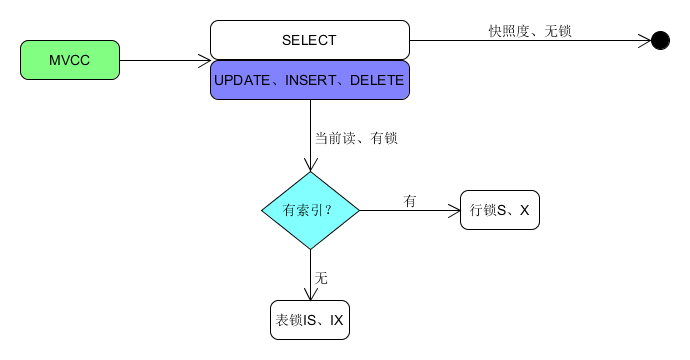
\includegraphics[width=15cm,height=7cm]{Index2}
			\caption{InnoDB 加锁主要逻辑}
		\end{figure}
	
		InnoDB与MyISAM的最大不同有两点:一是\textbf{支持事务(TRANSACTION)};二是\textbf{采用了行级锁}。行级锁和表级锁本来就有许多不同之处,另外,事务的引入也带来了一些新问题。
		
		\subsection{事务及其ACID属性}
			事务是\textbf{由一组SQL语句组成的逻辑处理单元},事务具有4属性,通常称为事务的ACID属性。
			
			\begin{itemize}
				\item \textbf{原子性(Actomicity)}:事务是一个原子操作单元,\textit{其对数据的修改,要么全都执行,要么全都不执行}。
				\item \textbf{一致性(Consistent)}:在事务开始和完成时,数据都必须保持一致状态。这意味着所有相关的数据规则都必须应用于事务的修改,以操持完整性;\textit{事务结束时,所有的内部数据结构(如B树索引或双向链表)也都必须是正确的}。
				\item \textbf{隔离性(Isolation)}:数据库系统提供一定的隔离机制,保证事务在不受外部并发操作影响的“独立”环境执行。这意味着\textit{事务处理过程中的中间状态对外部是不可见的},反之亦然。
				\item \textbf{持久性(Durable)}:事务完成之后,它\textbf{对于数据的修改是永久性的},即使出现系统故障也能够保持。
			\end{itemize}
		
		
		\subsection{并发事务带来的问题}
			相对于串行处理来说,并发事务处理能大大增加数据库资源的利用率,提高数据库系统的事务吞吐量,从而可以支持可以支持更多的用户。但并发事务处理也会带来一些问题,主要包括以下几种情况.
			
			\begin{itemize}
				\item \textbf{更新丢失(Lost Update)}:当两个或多个事务选择同一行,然后基于最初选定的值更新该行时,由于每个事务都不知道其他事务的存在,就会发生丢失更新问题——\textbf{最后的更新覆盖了其他事务所做的更新}。例如,两个编辑人员制作了同一文档的电子副本。每个编辑人员独立地更改其副本,然后保存更改后的副本,这样就覆盖了原始文档。最后保存其更改保存其更改副本的编辑人员覆盖另一个编辑人员所做的修改。\textit{如果在一个编辑人员完成并提交事务之前,另一个编辑人员不能访问同一文件,则可避免此问题}。
				\item \textbf{脏读(Dirty Reads)}:一个事务正在对一条记录做修改,\textbf{在这个事务并提交前},这条记录的数据就处于不一致状态;这时,\textit{另一个事务也来读取同一条记录,如果不加控制,第二个事务读取了这些“脏”的数据,并据此做进一步的处理,就会产生未提交的数据依赖关系}。这种现象被形象地叫做“脏读”。
				\item \textbf{不可重复读(Non-Repeatable Reads)}:一个事务在读取某些数据已经发生了改变、或某些记录已经被删除了!这种现象叫做“不可重复读”。
				\item \textbf{幻读(Phantom Reads)}:一个事务\textit{按相同的查询条件重新读取}以前检索过的数据,\textit{却发现}其他事务\textit{插入了满足其查询条件的新数据},这种现象就称为“幻读”。
			\end{itemize}
		
		
		\subsection{事务隔离级别}
			在并发事务处理带来的问题中,“更新丢失”通常应该是完全避免的。但防止更新丢失,并不能单靠数据库事务控制器来解决,需要应用程序对要更新的数据加必要的锁来解决,因此,\textbf{防止更新丢失应该是应用的责任}。
			
			\textit{“脏读”、“不可重复读”和“幻读”},其实\textbf{都是数据库读一致性问题},必须由数据库提供一定的事务隔离机制来解决。数据库实现事务隔离的方式,基本可以分为以下两种。
			
			\begin{itemize}
				\item 一种是\textbf{在读取数据前,对其加锁,阻止其他事务对数据进行修改}。
				\item 一种是\textbf{不用加任何锁},\textit{通过一定机制生成一个数据\underline{请求时间点}的一致性\underline{数据快照}(Snapshot),并用这个快照来提供一定级别(语句级或事务级)的一致性读取}。从用户的角度,好像是数据库可以提供同一数据的多个版本,因此,\textbf{这种技术叫做数据多版本并发控制}(\textbf{Multi-Version Concurrency Control},简称\verb|MVCC|或MCC),也经常称为\textbf{多版本数据库}。
			\end{itemize}
			
			\paragraph{MVCC}
				\url{https://blog.csdn.net/w2064004678/article/details/83012387}
				
			在MVCC并发控制中,读操作可以分成两类:\textbf{快照读 (snapshot read)}与\textbf{当前读 (current read)}。
			\begin{itemize}
				\item \textbf{快照读},读取的是记录的可见版本 (有可能是历史版本),\textbf{不用加锁}。
				\item \textbf{当前读},读取的是记录的\textit{最新版本},并且,当前读返回的记录,\textbf{都会加上锁},保证其他事务不会再并发修改这条记录。
			\end{itemize}
			
			
			在一个支持MVCC并发控制的系统中,哪些读操作是快照读?哪些操作又是当前读呢?以MySQL InnoDB为例:
			
			\paragraph{快照读}
				简单的\verb|select|操作,属于快照读,不加锁。(当然,也有例外)
				
				\verb|select * from table where ?; |
				
			\paragraph{当前读}
				\textit{特殊的读操作},\textit{插入/更新/删除}操作,属于当前读,\textbf{需要加锁}。
				
				下面语句都属于当前读,读取记录的最新版本。并且,读取之后,还需要保证其他并发事务不能修改当前记录,对读取记录加锁。其中,除了第一条语句,对读取记录加S锁 (共享锁)外,其他的操作,都加的是X锁 (排它锁)。
				
				\begin{lstlisting}
	select * from table where ? lock in share mode;
	select * from table where ? for update;
	insert into table values (…);
	update table set ? where ?;
	delete from table where ?;			
				\end{lstlisting}
				
			
			\paragraph{事务隔离级别}
				
				数据库的\textit{事务隔离越严格,并发副作用越小},但付出的代价也就越大,因为\textbf{事务隔离实质上就是使事务在一定程度上 “串行化”进行},这显然与“并发”是矛盾的。\textit{同时,不同的应用对读一致性和事务隔离程度的要求也是不同的,比如许多应用对“不可重复读”和“幻读”并不敏 感,可能更关心数据并发访问的能力}。
				
				为了解决“隔离”与“并发”的矛盾,ISO/ANSI SQL92定义了4个事务隔离级别,每个级别的隔离程度不同,允许出现的副作用也不同,应用可以根据自己的业务逻辑要求,通过选择不同的隔离级别来平衡 “隔离”与“并发”的矛盾。下表很好地概括了这4个隔离级别的特性。
				\begin{table}[H]
					\centering
					\caption{隔离级别}
					\begin{tabular}{p{5cm}<{\centering} | p{5cm}<{\centering} | p{1cm}<{\centering} |p{2.5cm}<{\centering} |p{1cm}<{\centering}}
						\toprule
						\diagbox[width=5cm,trim=l]{隔离级别}{允许的并发副作用}	& 读数据一致性 & 脏读 & 不可重复读 & 幻读\\
						\midrule
						未提交读 Read uncommitted &  最低级别,只能保证不读取物理上损坏的数据 & 是 & 是 & 是\\
						\hline
						已提交读 Read committed &  语句级 & 否 & 是 & 是 \\
						\hline
						可重复读 Repeatable read &  事务级 & 否 & 否 & 是 \\
						\hline
						可序列化 Serializable &  最高级别,事务级 & 否 & 否 & 否\\
						\bottomrule
					\end{tabular}
				\end{table}
		
		\subsection{InnoDB的行锁模式及加锁方法}
			\paragraph{锁分类}
			
				\subparagraph{行锁}
					InnoDB实现了以下两种类型的\textbf{行锁}。同样,数据库的锁就是读写锁的应用与管理。
		
					\begin{itemize}[itemindent = 1em]
						\item \textbf{共享锁(S):又称读锁}。允许一个事务去读一行,阻止其他事务获得相同数据集的排他锁。若事务T对数据对象A加上S锁,则事务T可以读A但不能修改A,其他事务只能再对A加S锁,而不能加X锁,直到T释放A上的S锁。这保证了其他事务可以读A,但在T释放A上的S锁之前不能对A做任何修改。
						\item \textbf{排他锁(X):又称写锁}。允许获取排他锁的事务更新数据,\textit{阻止其他事务取得相同的数据集共享读锁和排他写锁}。若事务T对数据对象A加上X锁,事务T可以读A也可以修改A,其他事务不能再对A加任何锁,直到T释放A上的锁。
					\end{itemize}
			
			
					对于共享锁,\textit{就是多个事务只能读数据不能改数据}。 
					
					对于排他锁,我当初就犯了一个错误,\textit{以为排他锁锁住一行数据后,其他事务就不能读取和修改该行数据},\textbf{其实不是这样的}。排他锁指的是一个事务在一行数据加上排他锁后,\textbf{其他事务不能再在其上加其他的锁}。mysql InnoDB引擎默认的修改数据语句:\textbf{update,delete,insert都会自动给涉及到的数据加上排他锁},\textit{select语句默认不会加任何锁类型},如果\textbf{加排他锁}可以使用select …for update语句,\textbf{加共享锁}可以使用select … lock in share mode语句。所以\textbf{加过排他锁的数据行在其他事务中是不能修改数据的},\textit{也不能}\textbf{通过for update和lock in share mode锁的方式查询数据},\textit{但可以}\textbf{直接通过select …from…查询数据,因为普通查询没有任何锁机制}。
			
				
				\subparagraph{表锁}	
					另外,为了允许行锁和表锁共存,实现多粒度锁机制,InnoDB还有两种内部使用的意向锁(Intention Locks),\textbf{这两种意向锁都是表锁}。
					
					\begin{itemize}[itemindent = 1em]
						\item \textbf{意向共享锁(IS)}:事务打算给数据行加共享锁,事务在给一个数据行加共享锁前必须先取得该表的IS锁。
						\item \textbf{意向排他锁(IX)}:事务打算给数据行加排他锁,事务在给一个数据行加排他锁前必须先取得该表的IX锁。
					\end{itemize}
				
				
					InnoDB行锁模式兼容性列表: 
					
					\begin{table}[H]
						\centering
						\caption{行锁模式兼容性}
						\begin{tabular}{p{5cm}<{\centering} | p{1cm}<{\centering} | p{1cm}<{\centering} |p{1cm}<{\centering} |p{1cm}<{\centering}}
							\toprule
							\diagbox[width=5cm,trim=l]{当前锁模式}{是否兼容/请求锁模式}	& X & IX & S & IS \\
							\midrule
								X	 & 冲突  &  冲突& 冲突 & 冲突 \\
							\hline
							 	IX & 冲突  & 兼容 &冲突  &  兼容\\
							\hline
								S &  冲突 & 冲突 & 兼容 & 兼容 \\
							\hline
								IS &  冲突 & 兼容 & 兼容 & 兼容 \\
							\bottomrule
						\end{tabular}
					\end{table}		
					
		  			如果一个\textbf{事务请求的锁模式}与\textbf{当前的锁}\underline{兼容},InnoDB\textbf{就请求的锁授予该事务};反之,如果两者两者不兼容,\textbf{该事务就要等待锁释放}。	
					
					\textbf{意向锁是InnoDB自动加的,不需用户干预}。对于\verb|UPDATE、DELETE和INSERT|语句,InnoDB\textbf{会自动}给涉及数据集\textbf{加排他锁(X)};对于普通SELECT语句,InnoDB不会加任何锁。 
				
				\subparagraph{显式加锁}
					事务可以通过以下语句显式给记录集加共享锁或排他锁:
					\begin{itemize}[itemindent = 1em]
						\item \textbf{共享锁(S)}:\verb|SELECT * FROM table_name WHERE ... LOCK IN SHARE MODE|
						\item \textbf{排他锁(X)}:\verb|SELECT * FROM table_name WHERE ... FOR UPDATE|
					\end{itemize}
			
					用\verb|SELECT ... IN SHARE MODE|获得\textbf{共享锁},\textit{主要用在需要数据依存关系时来确认某行记录是否存在,并确保没有人对这个记录进行UPDATE或者DELETE操作}。但是如果当前事务也需要对该记录进行更新操作,则很有可能造成死锁,\textit{对于锁定行记录后需要进行更新操作的应用,应该使用SELECT… FOR UPDATE方式获得排他锁}。
		
			\paragraph{获取InonoD行锁争用情况}
				可以通过检查\verb|InnoDB_row_lock|状态变量来分析系统上的行锁的争夺情况.
				
				\verb|show status like 'innodb_row_lock%';|
			
				\textbf{如果发现锁争用比较严重},如\verb|InnoDB_row_lock_waits|和\verb|InnoDB_row_lock_time_avg|的值比较高,还可以通过设置InnoDB Monitors来进一步观察发生锁冲突的表、数据行等,并分析锁争用的原因。
			
		\subsection{InnoDB行锁实现方式}
			InnoDB\textbf{行锁}是通过给索引上的索引项加锁来实现的,这一点MySQL与Oracle不同,后者是通过在数据块中对相应数据行加锁来实现的。InnoDB这种行锁实现特点意味着:\textbf{只有通过索引条件检索数据,InnoDB才使用行级锁,否则,InnoDB将使用\underline{表锁}}!
			
			在实际应用中,\textit{要特别注意InnoDB行锁的这一特性,不然的话,可能导致大量的锁冲突,从而影响并发性能}。下面通过一些实际例子来加以说明。
			
			\subsubsection{无索引-使用表锁}
				\begin{lstlisting}
	create table tab_no_index(id int,name varchar(10)) engine=innodb;
	insert into tab_no_index values(1,'1'),(2,'2'),(3,'3'),(4,'4');				
				\end{lstlisting}
				
				\begin{figure}[H]
					\centering
					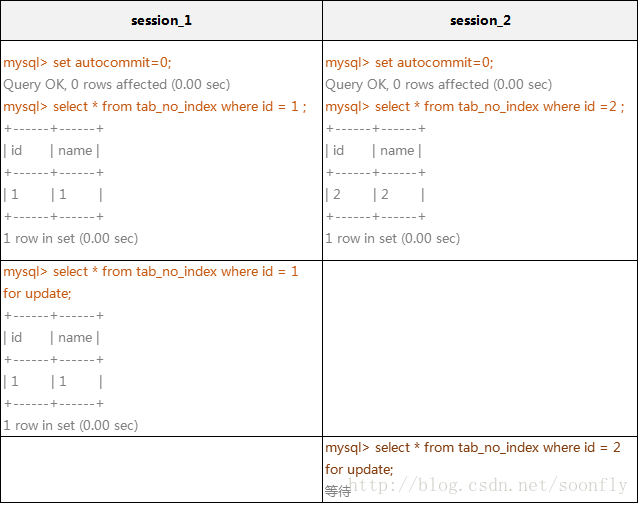
\includegraphics[width=13cm, height=13cm]{lock-table}
					\caption{无索引方式多进程加锁访问-类更新}
				\end{figure}
				
				在上面的例子中,看起来\verb|session_1|只给一行加了排他锁,但\verb|session_2|在请求其他行的排他锁时,却出现了锁等待!\textbf{原因就是在没有索引的情况下,InnoDB只能使用表锁}.
				
			\subsubsection{有索引-使用行锁-增加并发量}
				当我们\textbf{给其增加一个索引后},InnoDB就只锁定了符合条件的行,如下例所示: 
				\begin{lstlisting}
	create table tab_with_index(id int,name varchar(10)) engine=innodb;
	alter table tab_with_index add index id(id);			
				\end{lstlisting}
				
				\begin{figure}[H]
					\centering
					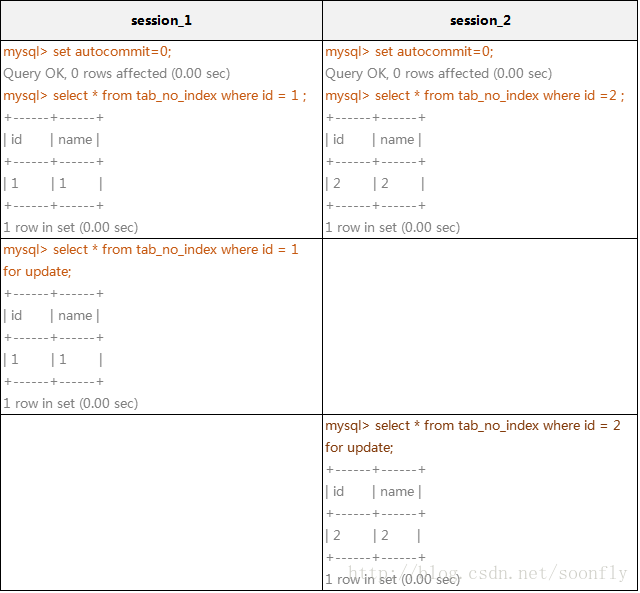
\includegraphics[width=13cm, height=15cm]{lock-row}
					\caption{有索引方式多进程加锁访问-类更新}
				\end{figure}
			
			
			\subsubsection{行锁-使用相同索引键值得等待锁}
				由于MySQL的行锁是\textbf{针对索引加的锁,不是针对记录加的锁},所以虽然是\textbf{访问不同行的记录,但是如果是使用相同的索引键,是会出现锁冲突的}。应用设计的时候要注意这一点。
			
				\begin{lstlisting}
	alter table tab_with_index drop index name;
	insert into tab_with_index  values(1,'4');	
	select * from tab_with_index where id = 1;
	id  names
	1 	1
	1	4		
				\end{lstlisting}
				
				InnoDB存储引擎使用相同索引键的阻塞例子
				
				\begin{figure}[H]
					\centering
					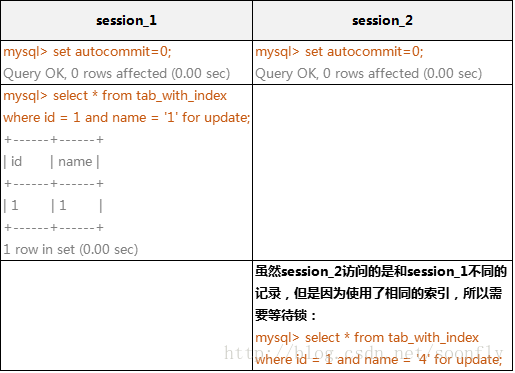
\includegraphics[width=13cm]{lock-row2}
					\caption{使用相同索引键-锁冲突}
				\end{figure}
			
			
			\subsubsection{行锁-使用不同的索引定位不同行也是行锁}	
				当表有多个索引的时候,不同的事务可以使用不同的索引锁定不同的行,另外,不论是使用主键索引、唯一索引或普通索引,InnoDB都会使用行锁来对数据加锁.
				
				\begin{lstlisting}
	alter table tab_with_index add index name(name);			
				\end{lstlisting}
			
				InnoDB存储引擎的表使用不同索引的阻塞例子 
				\begin{figure}[H]
					\centering
					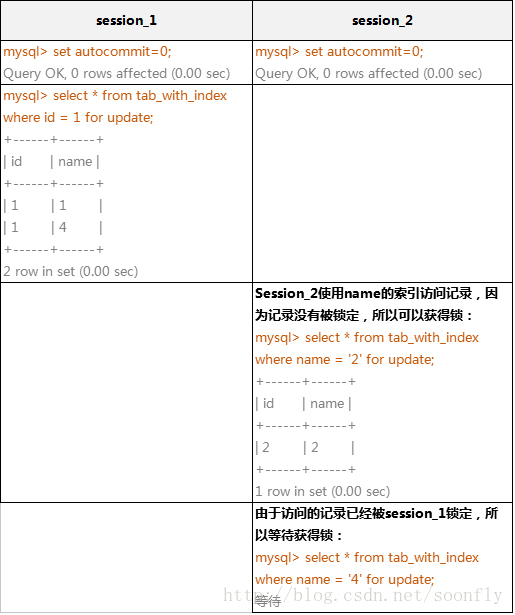
\includegraphics[width=13cm]{lock-row3}
					\caption{使用不同索引}
				\end{figure}				
			
			
			\subsubsection{是否真正使用索引}		
				即便在条件中使用了索引字段,\textbf{但是否使用索引来检索数据是由MySQL通过判断不同执行计划的代价来决 定的},如果MySQL认为全表扫描效率更高,比如对一些很小的表,它就不会使用索引,这种情况下InnoDB将使用表锁,而不是行锁。因此,\textbf{在分析锁冲突 时,别忘了检查SQL的执行计划},\textit{以确认是否真正使用了索引}。 
				
				比如,在\verb|tab_with_index|表里的\verb|name|字段有索引,但是\verb|name|字段是\verb|varchar|类型的,检索值的数据类型与索引字段不同,\textit{虽然MySQL能够进行数据类型转换,但却不会使用索引,从而导致InnoDB使用表锁}。\textbf{通过用explain检查两条SQL的执行计划,我们可以清楚地看到了这一点}。
				
				\begin{lstlisting}	
mysql> explain select * from tab_with_index where name = 1 \G
*************************** 1. row ***************************
           id: 1
  select_type: SIMPLE
        table: tab_with_index
   partitions: NULL
         type: ALL
possible_keys: name
          key: NULL
      key_len: NULL
          ref: NULL
         rows: 2
     filtered: 50.00
        Extra: Using where
1 row in set, 3 warnings (0.00 sec)

mysql> explain select * from tab_with_index where name = '1' \G
*************************** 1. row ***************************
           id: 1
  select_type: SIMPLE
        table: tab_with_index
   partitions: NULL
         type: ref
possible_keys: name
          key: name
      key_len: 33
          ref: const
         rows: 1
     filtered: 100.00
        Extra: NULL
1 row in set, 1 warning (0.00 sec)	
				\end{lstlisting}
				
			
		\subsection{间隙锁(Next-Key锁)}
			当我们\textbf{用范围条件}而\textbf{不是相等条件}检索数据,\textbf{并请求共享或排他锁时},InnoDB会\textbf{给符合条件的}已有数据记录的 \textbf{索引项加锁};\textit{对于键值在条件范围内但并不存在的记录},叫做“间隙(GAP)”,InnoDB\textbf{也会对这个“间隙”加锁},这种锁机制就是所谓的间隙锁 (Next-Key锁)。
			
			
			举例来说,假如\verb|emp表|中只有\verb|101|条记录,其\verb|empid|的值分别是\verb| 1,2,…,100,101|,下面的\verb|SQL|:
			\begin{lstlisting}
	Select * from  emp where empid > 100 for update;		
			\end{lstlisting}
			
			\textit{是一个范围条件的检索},\verb|InnoDB|\textbf{不仅会}对符合条件的\verb|empid值为101|的记录加锁,\textbf{而且会}对\verb|empid大于101|(这些记录并不存在)的\textbf{“间隙”加锁}。
			
			
			
			\paragraph{使用间隙锁的目的}
				
				\begin{itemize}
					\item 一方面是为了\textbf{防止幻读},以满足相关隔离级别的要求,对于上面的例子,\textit{要是不使 用间隙锁,如果其他事务插入了empid大于100的任何记录,那么本事务如果再次执行上述语句,就会发生幻读};
					\item 一方面,是为了\textit{满足}其 \textbf{恢复} 和 \textbf{复制}的需要。
				\end{itemize}
	
			很显然,在使用范围条件检索并锁定记录时,InnoDB这种加锁机制\textit{会阻塞符合条件范围内键值的并发插入,这往往会造成严重的锁等待}。因此,\textbf{在实际应用开发中,尤其是并发插入比较多的应用,我们要尽量优化业务逻辑,尽量使用相等条件来访问更新数据,避免使用范围条件}。
			
			
			\paragraph{特殊情况}
				还要特别说明的是,InnoDB除了通过范围条件加锁时使用间隙锁外,如果\textbf{使用相等条件请求给一个\underline{不存在的记录}加锁,InnoDB也会使用间隙锁}!
				
				下面这个例子假设\verb|emp表|中只有\verb|101|条记录,其\verb|empid|的值分别是\verb|1,2,……,100,101|。
				
				InnoDB存储引擎的间隙锁阻塞例子 
				\begin{figure}[H]
					\centering
					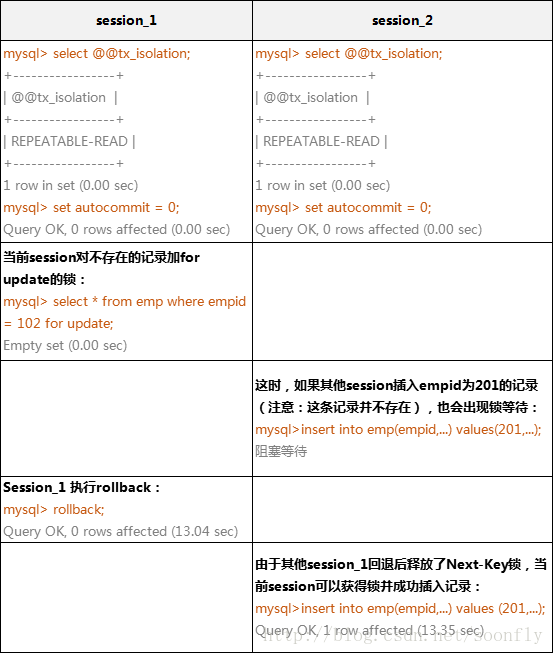
\includegraphics[width=13cm]{lock-next}
					\caption{间隙锁}
				\end{figure}			
				
				
		\subsection{什么时候使用表锁}
			对于InnoDB表,\textit{在绝大部分情况下都应该使用行级锁},因为\textbf{事务和行锁}往往\textit{是我们之所以选择InnoDB表的理由}。但\textbf{在个另特殊事务中,也可以考虑使用表级锁}。
			
			\begin{itemize}
				\item 第一种情况是:\textbf{事务需要更新大部分或全部数据},表又比较大,如果使用默认的行锁,不仅这个事务执行效率低,而且可能造成其他事务长时间锁等待和锁冲突,这种情况下可以考虑使用表锁来提高该事务的执行速度。
				\item 第二种情况是:\textbf{事务涉及多个表,比较复杂,很可能引起死锁,造成大量事务回滚}。这种情况也可以考虑一次性锁定事务涉及的表,从而避免死锁、减少数据库因事务回滚带来的开销。
			\end{itemize}
		
			当然,应用中\textbf{这两种事务不能太多,否则,就应该考虑使用MyISAM表}。
			
			在InnoDB下 ,使用表锁要注意以下两点。
			
			\begin{itemize}
				\item 使用\verb|LOCK TALBES|虽然\textbf{可以给InnoDB加表级锁},但必须说明的是,\textit{表锁不是由InnoDB存储引擎层管理的,而是由其上一层MySQL Server负责的},仅当\verb|autocommit=0|、\verb|innodb_table_lock=1|(默认设置)时,InnoDB层才能知道MySQL加的表锁,MySQL Server才能感知InnoDB加的行锁,这种情况下,InnoDB才能自动识别涉及表级锁的死锁;否则,InnoDB将无法自动检测并处理这种死锁。
				\item 在用\verb|LOCAK TABLES|对InnoDB锁时要注意,\textbf{要将AUTOCOMMIT设为0,否则MySQL不会给表加锁};事务结束前,不要用\verb|UNLOCAK TABLES|释放表锁,因为\verb|UNLOCK TABLES|\textbf{会隐含地提交事务};\verb|COMMIT|或\verb|ROLLBACK|产不能释放用\verb|LOCAK TABLES|加的表级锁,\textbf{必须用}\verb|UNLOCK TABLES|\textbf{释放表锁},正确的方式见如下语句。
				
				\begin{lstlisting}
	#例如,如果需要写表t1并从表t读,可以按如下做:	
	SET AUTOCOMMIT=0;
	LOCAK TABLES t1 WRITE, t2 READ, ...;
	[do something with tables t1 and here];
	COMMIT;
	UNLOCK TABLES;		
				\end{lstlisting}
				
			\end{itemize}
			
			
		\subsection{关于死锁}
			\verb|MyISAM|表锁是\verb|deadlock free|的,这是因为\verb|MyISAM|\textbf{总是一次性获得所需的全部锁,要么全部满足,要么等待},因此不会出现死锁。但是在\verb|InnoDB|中,\textbf{除单个}\verb|SQL|\textbf{组成的事务外,锁是逐步获得的},这就决定了\verb|InnoDB|发生死锁是可能的。
	
			\textit{发生死锁后},\textbf{InnoDB一般都能自动检测到,并使一个事务释放锁并退回,另一个事务获得锁,继续完成事务}。	
			\textit{但在涉及外部锁},\textit{或涉及锁的情况下},InnoDB\textbf{并不能完全}\textit{自动检测到死锁},这需要通过设置锁等待超时参数\verb|innodb_lock_wait_timeout|来解决。\textit{需要说明的是,这个参数并不是只用来解决死锁问题,在并发访问比较高的情况下,如果大量事务因无法立即获取所需的锁而挂起,会占用大量计算机资源,造成严重性能问题,甚至拖垮数据库}。我们通过设置合适的锁等待超时阈值,可以避免这种情况发生。
			
			通常来说,死锁都是应用设计的问题,通过调整业务流程、数据库对象设计、事务大小、以及访问数据库的SQL语句,绝大部分都可以避免。
			下面就通过实例来介绍几种避免死锁的常用方法。
			
			
			\begin{enumerate}
				\item 在应用中,\textbf{如果不同的程序会并发存取多个表,应尽量约定以相同的顺序为访问表,这样可以大大降低产生死锁的机会}。如果两个session访问两个表的顺序不同,发生死锁的机会就非常高!但如果以相同的顺序来访问,死锁就可能避免。
				\item 在程序以批量方式处理数据的时候,如果\textbf{事先对数据排序,保证每个线程按固定的顺序来处理记录},也可以大大降低死锁的可能。
				\item 在事务中,\textbf{如果要更新记录,应该直接申请足够级别的锁,即排他锁},而不应该先申请共享锁,更新时再申请排他锁,甚至死锁。
				\item 在\verb|REPEATEABLE-READ|隔离级别下,如果两个线程同时对相同条件记录用\verb|SELECT...ROR UPDATE|加排他锁,在没有符合该记录情况下,两个线程都会加锁成功。程序发现记录尚不存在,就试图插入一条新记录,如果两个线程都这么做,就会出现死锁。这种情况下,将隔离级别改成\verb|READ COMMITTED|,就可以避免问题。
				\item 当隔离级别为\verb|READ COMMITED|时,如果两个线程都先执行\verb|SELECT...FOR UPDATE|,\textit{判断是否存在符合条件的记录,如果没有,就插入记录}。此时,只有一个线程能插入成功,另一个线程会出现锁等待,当第1个线程提交后,第2个线程会因主键重出错,但\textbf{虽然这个线程出错了,却会获得一个排他锁}!这时如果有第3个线程又来申请排他锁,也会出现死锁。\textbf{对于这种情况,可以直接做插入操作,然后再捕获主键重异常,或者在遇到主键重错误时,总是执行ROLLBACK释放获得的排他锁}。
			\end{enumerate}
			
			尽管通过上面的设计和优化等措施,可以大减少死锁,但死锁很难完全避免。因此,\textbf{在程序设计中总是捕获并处理死锁异常}是一个很好的编程习惯。
			
	\section{总结}
		\subsection{MyISAM}
			\begin{enumerate}
				\item 共享读锁(S)之间是兼容的,但共享读锁(S)和排他写锁(X)之间,以及排他写锁之间(X)是互斥的,也就是说读和写是串行的。
				\item 在一定条件下,MyISAM允许查询和插入并发执行,我们可以利用这一点来解决应用中对同一表和插入的锁争用问题。
				\item MyISAM默认的锁调度机制是写优先,这并不一定适合所有应用,用户可以通过设置\verb|LOW_PRIPORITY_UPDATES|参数,或在\verb|INSERT|、\verb|UPDATE|、\verb|DELETE|语句中指定\verb|LOW_PRIORITY|选项来调节读写锁的争用。
				\item \textbf{由于表锁的锁定粒度大,读写之间又是串行的},因此,如果更新操作较多,MyISAM表可能会出现严重的锁等待,可以考虑采用InnoDB表来减少锁冲突。
			\end{enumerate}
		
		
		\subsection{InnoDB}
			\begin{enumerate}
				\item InnoDB的行锁是基于索引实现的,如果不通过索引访问数据,InnoDB会使用表锁。
				\item InnoDB间隙锁机制,以及InnoDB使用间隙锁的原因。
				\item 在不同的隔离级别下,InnoDB的锁机制和一致性读策略不同。
				\item MySQL的恢复和复制对InnoDB锁机制和一致性读策略也有较大影响。
				\item 锁冲突甚至死锁很难完全避免。
			\end{enumerate}
			
			在了解InnoDB的锁特性后,用户可以通过设计和SQL调整等措施减少锁冲突和死锁,包括:
			\begin{itemize}
				\item 尽量使用较低的隔离级别
				\item 精心设计索引,并尽量使用索引访问数据,使加锁更精确,从而减少锁冲突的机会。
				\item 选择合理的事务大小,小事务发生锁冲突的几率也更小。
				\item 给记录集显示加锁时,最好一次性请求足够级别的锁。比如要修改数据的话,最好直接申请排他锁,而不是先申请共享锁,修改时再请求排他锁,这样容易产生死锁。
				\item 不同的程序访问一组表时,应尽量约定以相同的顺序访问各表,对一个表而言,尽可能以固定的顺序存取表中的行。这样可以大减少死锁的机会。
				\item 尽量用相等条件访问数据,这样可以避免间隙锁对并发插入的影响。
				\item 不要申请超过实际需要的锁级别;除非必须,查询时不要显示加锁。
				\item 对于一些特定的事务,可以使用表锁来提高处理速度或减少死锁的可能。
			\end{itemize}
		
		
\chapter{日志}
	
	\begin{table}[H]
		\centering
		\caption{日志功能选项配置说明}
		\begin{tabular}{p{9cm} | p{7cm}}
			\toprule[1.5pt]
				选项  &   用途 	\\
			\midrule
				\verb| general_log | &  启用\textbf{普通日志}	\\
				\verb| general_log_file=file_name | & 生成日志文件名  	\\
				\verb| log-bin[=file_name] | &  	启用\textbf{二进制日志} \\
				\verb| log-bin-index=file_name | &  二进制日志索引文件	\\
				\verb| log_error[=file_name] | &   启用\textbf{出错日志}	\\
				\verb| log_output[=destination] | &  普通查询/慢查询 日志存在位置	\\
				\verb| relay-log[=file_name] | &  启用\textbf{中继日志}	\\
				\verb| relay-log-index=file_name | &  中继日志索引文件	\\
				\verb| slow_query_log | &  启用\textbf{慢查询日志}	\\
				\verb| slow_query_log_file=file_name | &  慢查询日志文件名	\\
			\bottomrule[1.5pt]
		\end{tabular}
	\end{table}
	
	
	\section{error-log}
		这种日志记录的内容包括服务器的启动和关闭、以及与问题或异常条件有关的消息。 
		
		如果服务器无法启动,就可以查看此类日志,它会在终止之前把消息写到出错日志,以指明出现了什么问题。
		
	\section{general-log}
		常规查询日志 包含的是:与服务器操作有关的常规信息。其中包括谁连接服务器、从什么地方连接、调用了哪些语句。	
		
		
	
	\section{slow-query-log}
		这种日志可以帮你把那些可能需要被重写,以求获得更好性能的语句识别出来。
	
		MySQL \textbf{慢查询日志}是指 MySQL 中\textbf{执行时间超过} \verb|long_query_time| \textbf{阀值的 SQL 语句}。
		
		\verb|Dumbo| 默认每天零晨 \textbf{rotate 慢查询日志},按日期命名文件,每天一个文件,服务器上保留最近 8 天的慢查询日志文件。
		
		\textit{从慢查询日志中统计出执行比较频繁且执行时间比较久、扫描的行数也比较大的 SQL,可以针对这类 SQL 进行优化。}
	
		\paragraph{参数说明}
			慢查询日志相关的几个参数,有先后依赖关系,顺序如下:
			\begin{enumerate}[itemindent = 2em, itemsep = 0pt,partopsep=0pt]
				\item \verb|slow_query_log| \\ 是否启用慢查询日志功能,慢查询日志的内容可以在 \textbf{Dumbo 管理平台} \textit{实例管理 --> 日志管理 --> 慢查询日志} 上查看
				\item \verb|log_slow_admin_statements| \\ 是否记录administrative statements 语句到慢查询日志里。
				\item \verb|long_query_time| \\ 定义慢查询日志的触发条件,如果 SQL 实际执行时间(不包括锁的时间)超过 \verb|long_query_time| 定义的阀值,此 SQL 则被记录到慢查询日志里。
				\item \verb|min_examined_row_limit| \\ 只有慢查询语句的执行行数检查返回大于该参数指定值,此慢查询语句才被记录到慢查询日志中。
			\end{enumerate}
			
			\begin{table}[H]
				\centering
				\caption{慢查询日志参数}
				\begin{tabular}{p{5.5cm}<{\centering}|p{3cm}<{\centering}|p{3cm}<{\centering}|p{3cm}<{\centering}}
					\hline
						方法 &  MySQL默认值 &  Dumbo 默认值 & 能否自助修改\\
					\hline
				 \verb|slow_query_log| & OFF & ON &  否 \\
				 \verb|long_query_time| & 10s & 0.1s & 能 \\
				 \verb|log_slow_admin_statements| & OFF & ON & 否 \\
				 \verb|log_slow_slave_statements| & OFF & ON &否\\
				 \verb|min_examined_row_limit| & 0& 100 & 否 \\
					\hline
				\end{tabular}					
			\end{table}
			
			
			因此 \textbf{Dumbo 实例默认配置下},记录慢查询日志的条件是:
			\textbf{SQL 实际执行时间超过 0.1s,且此 SQL 的执行行数检查返回值大于 100}。
		\paragraph{优点}
			\begin{itemize}
				\item 语句调优 \\ 通过统计慢查询日志(可联系 Dumbo 值班),找出最耗时的 top 10 语句,优化完成后,再统计新的慢查询日志,一直重复,直到没有产生新的慢查询语句。
				\item 性能排查 \\ 如果一个实例的 CPU 使用率比较高,可以优先检查一下该实例的慢查询日志,如果慢查询日志刷得比较厉害,可以初步确认是由于 SQL 语句不够优化导致实例 CPU 使用率高,可以通过优化 SQL 来解决。
			\end{itemize}
		
		\paragraph{参考}
			\begin{itemize}
				\item \url{https://www.cnblogs.com/saneri/p/6656161.html}
			\end{itemize}
			
	\section{bin-log}
		这种日志由一个或多个文件构成,\textbf{记录}由\verb@UPDATE DELETE INSERT CREATE|DROP(TABLE) GRANT@ 等语句所做的\textbf{修改}。
		写到二进制日志里的内容都是一些\textbf{以二进制格式编码的数据修改“事件”}。 二进制日志文件都伴随有一个索引文件,其中列出了当时存在的那些二进制日志文件。
		
		MySQL的二进制日志可以说是MySQL\textbf{最重要的日志}了,它记录了所有的\textbf{DDL和DML}(除了数据查询语句)语句,\textbf{以事件形式记录,还包含语句所执行的消耗的时间},MySQL的二进制日志是事务安全型的。
		
		二进制有两个最重要的使用场景: 
			\begin{itemize}
				\item 其一:MySQL Replication\textbf{在Master端开启binlog},\textit{Master把它的二进制日志传递给slaves}来达到master-slave数据一致的目的。 
				\item 其二:是数据恢复,通过使用mysqlbinlog工具来使恢复数据。首先,根据备份文件恢复数据库,然后,使用mysqlbinlog 将二进制日志的内容转换为文本语句,并使用备份之后修改数据库的那些语句作为客户端mysql 的输入,把数据库恢复到崩溃时的状态。
			\end{itemize}    
		    
		\subparagraph{参考}
			\url{https://www.cnblogs.com/martinzhang/p/3454358.html}		
	
	
	\section{relay-log}
		中继日志。
		
		如果服务器是一个复制从服务器, 它就会维护一个中继日志,其中包含的是从主服务器接收到的需要被执行的数据修改事件记录。
		
		中继日志文件的格式与二进制日志文件的格式相同,它有一个索引文件,其中列出的是从服务器器上存在的日志文件。
	
	
	\section{redo-log}
		\url{https://www.cnblogs.com/f-ck-need-u/archive/2018/05/08/9010872.html}
		
		redo log通常是物理日志,记录的是数据页的物理修改,而不是某一行或某几行修改成怎样怎样,它用来恢复提交后的物理数据页(恢复数据页,且只能恢复到最后一次提交的位置)。
	
	
	\section{undo-log}
		undo用来回滚行记录到某个版本。undo log一般是逻辑日志,根据每行记录进行记录。
		
	
	\section{日志表}
		当启用了普通查询日志或慢查询日志功能时,你可以选择让服务器把日志输出写入日志文件、写入MySQL 数据库的日志表,或同时写入这两个地方。
		
		如果把\verb|TABLE |作为输出目标,服务器会把日志输出写入 mysql 数据库的 \verb|general_log |和 \verb|slow_log |表。
		
		如果把\verb|FILE |作为输出目标,日志文件名就由全局系统变量 \verb|general_log_file| 和 \verb|slow_query_log_file| 来决定。文件位于数据目录里,默认名分别为 \verb|HOSTNAME.log| 和 \verb|HOSTNAME-slow.log|.
		
\chapter{存储引擎}
	\section{InnoDB存储引擎}	
	
	
\chapter{集群} 
	\section{备份-重要}
		\begin{itemize}
			\item mysqldump: 逻辑备份; 单线程导入导出; 注意设定字符集; 
			\item mydumper: 逻辑备份; “多线程”导入导出; 无需关心字符集;
			\item innobackup/mysqlbackup: 物理备份; 速度较快;
		\end{itemize}
		\subsection{普通数据库备份}
			\verb|mysqldump -u root -p password --default-character-set=utf-8 dataname > dataname.sql|
			
			\verb|mysql -u root -p password --default-character-set=utf-8 dataname < dataname.sql|
		\subsection{备份到压缩文件}
			\verb@mysqldump -u root -p database | gzip > database.sql.gz@
			
			\verb@gzip < database.sql.gz | mysql -u root -p database@
		\subsection{增量备份}
			\verb@mysqlbinlog bin-log.000002 |mysql -uroot -ppassword@
		

	\section{主从模式-replication}
	
	\section{集群}


\chapter{PHP 与 MySQL}


\chapter{MySQL 性能优化}
	\begin{figure}[H]
		\centering
		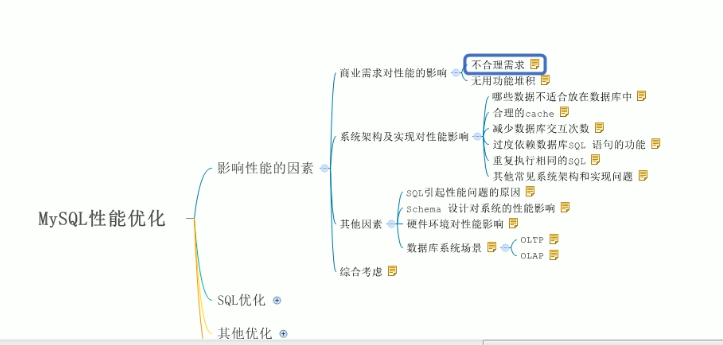
\includegraphics[scale=0.7]{xingNeng}
		\caption{性能优化结构}
	\end{figure}
	
	
	\url{https://www.cnblogs.com/kenmeon/p/9770998.html}
	
	
	\section{影响性能的因素}
		\subsection{不合理的需求如何优化}
			需求: 一个论坛帖子总量的统计
			附加要求:实时更新
			
			\begin{itemize}
				\item 初始阶段:\verb|select count(id)|
				\item 新建一个表,在这个表中更新这个汇总数据 (频率问题- update 锁)
				\item 真正的问题在于,实时?创建一个统计表,隔一段时间统计一次并存入(Redis)。
			\end{itemize}
		
		\subsection{无用功能的堆积}
			\begin{itemize}
				\item 无用的列堆积
				\item 错误的表设计
				\item 无用的表关联
			\end{itemize}
		
		
		\subsection{哪些数据不适合放在数据库中}
			\begin{itemize}
				\item 二进制文件-文件-图片
				\item 流水队列数据
				\item 超大文本
			\end{itemize}
		
		
		\subsection{合理的cache}
			哪些数据适合放到cache 中
			\begin{itemize}
				\item 系统的配置信息 
				\item 活跃用户的基本信息 
				\item 活跃用户的定制化信息
				\item 基于时间段的统计信息
				\item 读 >>> 写的数据
			\end{itemize}
		
		\subparagraph{减少数据库交互次数}
		\subparagraph{减少重复执行相同的SQL}
	
		\subsection{其他}
			\begin{itemize}
				\item cache 系统的不合理利用导致Cache 命中率底下造成的数据库访问量的增加,同事也浪费了Cache系统的硬件资源投入
				\item 过度依赖面向对象思想,对系统的可扩展性的过度追求,促使系统设计的时候将对象拆的过于分散,造成系统中大量的复杂join 语句,而MySQL 在各数据库系统中的主要优势在于处理简单逻辑的查询,这与其锁定的机制也有较大关系
				\item 对数据库过度依赖,将大量适合存放于文件系统中的数据存入了数据库中,造成数据库资源的浪费,影响到系统的整体性能,如各种日志信息
				\item 过度理想化系统的用户体验,是大量的非核心业务消耗过多的资源,如大量
			\end{itemize}
			
	\section{Sql 优化}	
		
		
	\section{Explain 详解}
		\url{https://www.cnblogs.com/xuanzhi201111/p/4175635.html}
		
		\url{https://www.cnblogs.com/galengao/p/5780958.html}
		
		在日常工作中,我们会有时会开慢查询去记录一些执行时间比较久的SQL语句,找出这些SQL语句并不意味着完事了,些时我们常常用到explain这个命令来查看一个这些SQL语句的执行计划,查看该SQL语句有没有使用上了索引,有没有做全表扫描,这都可以通过explain命令来查看。
		
		expain出来的信息有10列,分别是\verb|id|、\verb|select_type|、\verb|table|、\verb|type|、\verb|possible_keys|、\verb|key|、\verb|key_len|、\verb|ref|、\verb|rows|、\verb|Extra|,下面对这些字段出现的可能进行解释:
		
		\subsection{id}
			SQL执行的顺序的标识,SQL从大到小的执行
			\begin{itemize}
				\item id相同时,执行顺序由上至下
				\item 如果是子查询,id的序号会递增,id值越大优先级越高,越先被执行
				\item id如果相同,可以认为是一组,从上往下顺序执行;在所有组中,id值越大,优先级越高,越先执行
			\end{itemize}
			
		\subsection{select\_type}
			\begin{itemize}
				\item \verb|SIMPLE|  :简单SELECT,不使用UNION或子查询等
				\item \verb|PRIMARY| :查询中若包含任何复杂的子部分,最外层的select被标记为PRIMARY
				\item \verb|UNION| :UNION中的第二个或后面的SELECT语句
				\item \verb|DEPENDENT UNION| :UNION中的第二个或后面的SELECT语句,取决于外面的查询
				\item \verb|UNION RESULT| :UNION的结果
				\item \verb|SUBQUERY| :子查询中的第一个SELECT
				\item \verb|DEPENDENT SUBQUERY| :子查询中的第一个SELECT,取决于外面的查询
				\item \verb|DERIVED| :派生表的SELECT, FROM子句的子查询
				\item \verb|UNCACHEABLE SUBQUERY| :一个子查询的结果不能被缓存,必须重新评估外链接的第一行
			\end{itemize}
			
		\subsection{table}	
			显示这一行的数据是关于哪张表的
			
		\subsection{type}
			
			\begin{itemize}
				\item \verb|ALL|:Full Table Scan, MySQL将\textbf{遍历全表}以找到匹配的行
				\item \verb|Index|: Full Index Scan,index与ALL区别为index类型\textbf{只遍历索引树}
				\item \verb|Range|:只检索给定范围的行,使用一个索引来选择行
				\item \verb|Ref|: 表示上述表的连接匹配条件,即哪些列或常量\textbf{被用于查找索引列上的值}
				\item \verb|Eq_ref|: 	类似ref,区别就在使用的索引是唯一索引,对于每个索引键值,表中只有一条记录匹配,简单来说,就是多表连接中使用primary key或者 unique key作为关联条件
				\item \verb|Const|、\verb|System|: 当MySQL对查询某部分进行优化,并转换为一个常量时,使用这些类型访问。如将主键置于where列表中,MySQL就能将该查询转换为一个常量,system是const类型的特例,当查询的表只有一行的情况下,使用system
				\item \verb|NULL|: MySQL在优化过程中分解语句,执行时甚至不用访问表或索引,例如从一个索引列里选取最小值可以通过单独索引查找完成。
			\end{itemize}
			
		\subsection{possible\_keys}
			指出MySQL能使用哪个索引在表中找到记录,查询涉及到的字段上若存在索引,则该索引将被列出,但不一定被查询使用
			
		\subsection{Key}
			key列显示MySQL实际决定使用的键(索引)
			
		\subsection{key\_len}
			表示索引中使用的字节数,可通过该列计算查询中使用的索引的长度(\verb|key_len|显示的值为索引字段的最大可能长度,并非实际使用长度,即\verb|key_len|是根据表定义计算而得,不是通过表内检索出的)
			
			不损失精确性的情况下,长度越短越好 
			
		\subsection{ref}
			表示上述表的连接匹配条件,即哪些列或常量被用于查找索引列上的值
			
		\subsection{rows}
			表示MySQL根据表统计信息及索引选用情况,估算的找到所需的记录所需要读取的行数
	
		\subsection{filtered}
			Percentage of rows filtered by table condition
			
			它指\textit{返回结果的行}占\textit{需要读到的行}(rows列的值)的\textbf{百分比}。按说filtered是个非常有用的值,因为对于join操作,前一个表的结果集大小直接影响了循环的次数。但是我的环境下测试的结果却是,filtered的值一直是100\%,也就是说失去了意义。
			
		\subsection{总结}
			\begin{itemize}
				\item EXPLAIN\textbf{不会}告诉你关于触发器、存储过程的信息或用户自定义函数对查询的影响情况
				\item EXPLAIN\textbf{不考虑}各种Cache
				\item EXPLAIN\textbf{不能}显示MySQL在执行查询时所作的优化工作
				\item \textbf{部分}统计信息\textbf{是估算的},并非精确值
				\item EXPALIN\textbf{只能}解释\verb|SELECT操作|,其他操作要重写为SELECT后查看执行计划。
			\end{itemize}
			

	\section{查询优化-海量数据}
	
	\section{经验Tips}
		\url{https://coolshell.cn/articles/1846.html}
		
		\begin{enumerate}
			\item \textbf{EXPLAIN} \verb|SELECT| 查询 \\ 解释查询语句,查看是否使用到索引(\textbf{Key})
			\item 当只要一行数据时使用 \verb|LIMIT 1|  \\ 这样会在找到一条数据后停止搜索,而不是继续往后查少下一条符合记录的数据
			\item 为搜索字段建索引 \\ BTree Or Hash Better Than All
			\item 在Join表的时候使用相当类型的例,并将其索引
			\item 千万不要 \verb|ORDER BY RAND()|
			\item 避免 \verb|SELECT *|
			\item 永远为每张表设置一个ID
			\item 使用 \verb|ENUM| 而不是 \verb|VARCHAR|
			\item 尽可能的使用 \verb|NOT NULL|
			\item 无缓冲的查询
			\item 把IP地址存成 \verb|UNSIGNED INT|
			\item 固定长度的表会更快
			\item 垂直分割
			\item 拆分大的 DELETE 或 INSERT 语句
			\item 越小的列会越快
			\item 选择正确的存储引擎
		\end{enumerate}

\chapter{数据库设计}
	\section{E-R 图}

		

\chapter{MySQL 管理}
	\section{MySQL组件}
		\subsection{Mysql 服务器}
			服务器主程序mysqld, 是MYSQL 数据系统的核心。 负责管理所有数据库和表。
		
		\subsection{Mysql 客户端}
			\begin{itemize}
				\item \verb|mysql| 一个交互程序,用来向服务器发送SQL语句,和查看结果。
				\item \verb|mysqladmin| 用于完成许多任务、如关闭服务器、检查配置、在运行不正常时监视状态。
				\item \verb|mysqldump| 用于备份数据库、或把数据库复制到另一个服务器的工具。
				\item \verb|mysqlcheck和myisamchk| 能帮你完成表的检查、分析、优化,还能修复受损表。 主要适用于 myisam 表。
			\end{itemize}
		
		\subsection{服务器语言SQL}
		
		\subsection{MySQL 数据目录}
			服务器会把数据库和状态文件存储在数据目录里。 
		
			查看数据目录的方法:
			\begin{itemize}[itemindent = 1em]
				\item 在配置文件\verb|[mysqld] -> datadir=···|
				\item 进入Mysql \verb|SHOW VARIABLES LIKE 'datadir'|
				\item \verb|mysqladmin variables|
			\end{itemize}
			
			\paragraph{数据目录结构}
				\begin{itemize}
					\item 每个数据库在数据目录下都对应有一个数据库目录。
					\item 数据库里的表、视图、触发器 都对应于数据库目录中的文件。
					\item 数据目录也可以包含其他文件,如进程id文件、服务器生成的状态文件、日志、等文件
				\end{itemize}
				
			
			\paragraph{数据访问方式}
				服务器是访问数据库的唯一联络点,它好像是处于客户端程序和他们想要使用的数据之间的中间人。
				
				\begin{figure}[H]
					\centering
					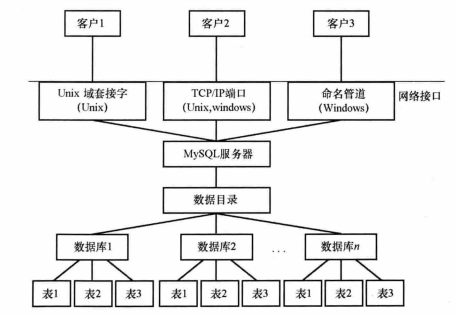
\includegraphics[width=15cm,height=10cm]{datadir}
					\caption{服务器控制数据目录访问的方式}
				\end{figure}
			
			\paragraph{数据库在文件系统里的表示}
				每个数据库都有其自己的数据库目录。
				
				\verb|show databases;| 语句可以列出位于数据目录里的目录名称。
				
				\verb|create database db_name| 语句会在数据目录下创建一个名为 \verb|db_name| 的数据库目录。
			
				\verb|drop databse db_name| 语句 则相当于执行了\verb|rm -rf datadir/db_name |.
				
			\paragraph{表在文件系统里的表示}
				对于一个表,Mysql 在磁盘上至少会\textbf{使用一个文件来表示},既\verb|.frm| 格式文件。
				
				服务器会负责创建\verb|.frm|文件, 而各个存储引擎会创建一些附加文件, 用于保存数据行和索引信息。这些文件的名字和结构会因存储引擎的不同而有所差异。
				
				在InnoDB 中,可以实现每个表一个表空间的存储模式,在这种情况下,每个InnoDB 表在数据库目录里都会有两个与表特定相关的文件。既\verb|.frm|文件 和 \textbf{包含表数据和索引的} \verb|.ibd|文件. 
				
				
			\paragraph{视图和触发器 在 文件系统里的表示}
			
				每个视图只有一个\verb|.frm|文件,其中包含着该视图的定义和其他相关属性,该文件的名称与视图的名称保持一致。
				
				每个触发器存储在一个\verb|.TRG|文件里,其中包含着该触发器的定义和其他相关属性,该文件的名称与触发器\textbf{关联表的名称}保持一致。
				如果一个表有多个触发器,那么服务器会把他们的所有定义集合存储在一个\verb|.TRG|文件里。每个触发器还有一个根据触发器名称命名的\verb|.TRN| 文件。
			
			
			\paragraph{状态文件 和 日志文件}
				数据目录还包括许多状态文件和日志文件。这些文件的默认位置为服务器的数据目录。 默认名称是从表中表示为\verb|HOSTNAME|的服务器主机名继承来的。
				
				二进制日志 和 中继日志 都会被创建为一组带编号的文件。
			
			
			\paragraph{影响表最大长度的因素}
				在mysql 里,表的长度是有限的,不过表的长度受很多方面的限制。除了受操作系统的限制以外,MySQL表的长度还受其自己内部限制。这些内部限制会因不同的存储引擎而有所不同。
			
					
				
			\paragraph{数据目录结构对系统性能的影响}
				每个表在数据目录里对应的文件个数,成为性能影响的点,因为在操作这个表时,系统必须为其分配一个文件描述符。因而不同的存储引擎如InnoDB(2个) 与 Myisam(3个) 就表现的不同。
				
				
		
		\subsection{迁移MySQL 数据目录}
			迁移方法总结
			
			\begin{table}[H]
				\centering
				\caption{迁移方法总结}
				\begin{tabular}{p{8cm}<{\centering} | p{7cm}<{\centering}}
					\toprule[1.5pt]
						迁移实体  &  适用的迁移方法\\
					\midrule
						\textbf{整个}数据目录 & 启动选项 Or 符号链接 \\
						\textbf{各个数据库}目录 & 符号链接 \\
						\textbf{各个数据库表} & 符号链接 \\
						\verb|InnoDB| 表空间文件 & 启动选项  \\
						服务器\verb|PID文件| & 启动选项  \\
						日志文件 & 启动选项  \\
					\bottomrule[1.5pt]
				\end{tabular}
			\end{table}
		
				
	\section{常规管理}
		参考<Mysql 技术内幕-美10.2>
		
		\subsection{用户账户维护}
			Mysql 上已有账户全部都列在\verb|mysql| 数据库 的 \verb|user| 表里。	
		
		\subsection{服务器的启动与关闭}
			应该以root 以外的其他用户身份来运行服务器,应该对所有进程的权限进行限制,除非它真的需要root 权限(mysqld 不需要)。
			
			每次都应该以同一个用户身份来运行服务器。当服务器不定时以不同用户权限运行时,会出现权限不一致的问题。这时,数据目录里创建的文件和目录会拥有不同的所属模式,会导致服务器在以某个用户身份运行时无法访问某些数据库和表。只有固定以同一个用户身份运行服务器,才能避免这个问题。
			
			
			\textbf{启动服务器}\verb|mysqld --verbose --help| or \verb|mysqld_safe| or \verb|mysqld.server| or \verb|mysqld_multi|
			
			\textbf{停止服务器}\verb|mysqladmin -p -u root shutdown| or \verb|/etc/init.d/mysql stop|
		
		
		\subsection{系统变量和状态变量}
			\paragraph{系统变量}
			
				\verb|show variables;|
				
				一个系统变量可以同时拥有全局值 和 会话值、只拥有一个全局值、或者只拥有一个会话值。
				
				当然还可以\textbf{利用正则查找相关的变量},如\verb|show variables like '%log%';|。当然也可以使用 \verb|where| 语句。
				
				\verb|SHOW variables WHERE Variable_name LIKE '%timeout%' AND Value < 60;|
				
				默认情况下,\verb|SHOW VARIABLES;| 会显示各个会话变量值,要想特定地显示全局变量或会话变量,可以在语句中加上\verb|GLOBAL|或\verb|SESSION|.
				
				\verb|SHOW GLOBAL VARIABLES; 	SHOW SESSION VARIABLES;|
				
				
				如果要查看当个变量值,可以使用语法格式  \verb|@@GLOBAL.var_name| 或\verb|@@SESSION.var_name|. 如果没有指定限定符,既\verb|@@var_name|  使用的是会话变量。这种一般配合\verb|SELECT |使用。
				
				
				\verb|select @@sql_mode;|
				
				这些变量在系统未启动前,可以通过修改配置文件修改,但是当系统运行时,需要借助\verb|SET|来完成设置。
				
				\verb|SET GLOBAL var_name = value;       SET @@GLOBAL.var_name = value;|
				
				当然,如果没有限定符号,那么\verb|SET|语句会修改的是当前会话。
				
				\verb|SET var_name = value;|
				
			\paragraph{状态变量}用于监视服务器运作情况。
			
				\verb|show status;|
						
				状态变量只能由服务器来设置,对于用户来说,只能查看。
				
				
			
		\subsection{日志维护-管理}
			服务器可以生成多种类型的日志,这些日志有助于诊断问题,提高性能、启用复制、恢复崩溃。
			
			确保最近的几个日志可以在线使用,同事还想放置日志文件无限制的增长,可以使用日志文件过期技术。
			
			\begin{itemize}
				\item \textbf{日志轮换法}
					
					这种方法适用于文件名固定的日志文件,如出错日志文件、普通查询日志文件和慢查询日志文件。
					
				\item \textbf{基于使用期限的过期法}
				
					这种方法会把超过某个使用期限的日志文件删除掉,它适用于按编号顺序创建的日志文件。不过,如果把二进制日志用于服务器复制,就不应该使用这种技术。
					
				\item \textbf{与复制有关的过期法}
				
					如果把二进制日志文件用于服务器复制,不能基于使用期限让他们过期。只有在知道他们都一倍完全发送至所有从服务器之后,才可以让其过期。因此,这种形式的过期方法是一句哪些二进制日志文件仍在使用来决定的。
					
					复制从服务器会按照编号顺序来创建中继日志文件,并且会在处理完他们之后自动将其删除。为减少存储在磁盘上的中继日志信息量,可以通过减小系统变量\verb|max_relay_log_size|的值来降低日志文件的最大可允许大小。
					
				\item \textbf{日志表截断或轮换法}
					
					如果把日志信息记录到mysql 数据库的表,就可以把它们截短或者重新命名,并将其替换为空表。
			\end{itemize}
		
		
		\subsection{服务器配置和优化}
		
		
		
		
		\subsection{管理多个服务器}
		
		
		
		\subsection{更新Mysql软件}
	
	
	
	
	\section{数据库维护、备份、复制}
		
		\subsection{预防性维护}
		
		\subsection{数据库备份}
			当出现严重的服务器崩溃事件时,数据库备份能起到关键的作用。在数据库崩溃之后,你肯定会希望把数据库恢复到崩溃前的状态,同时尽可能减少数据损失。
			
			在进行系统备份时,表所对应的文件很可能因服务器的活动而处于变化状态,因此恢复哪些文件并不能保证表的一致性。对于恢复数据库而言,mysqldump 程序生成的备份文件会更有用。
			
		\subsection{崩溃恢复}
			一定要知道\textbf{如何利用备份文件}来恢复数据、以及\textbf{如何利用二进制日志}恢复最近一次备份后所发生的那些更改。
			
		\subsection{数据库迁移}
			如果打算把现有的MySQL 迁移到一台速度更快的主机上,那么需要把数据库复制到另一台机器上。此过程需要熟悉整个流程的操作、以及过程的依赖条件、系统环境等。
			
		\subsection{数据库复制}
			主从复制。对数据库进行备份或制作副本。
		
\chapter{疑难杂症}
	\section{mysql.sock -ERROR 2002 (HY000)}
		
		\verb|Can't connect to local MySQL server through socket '/tmp/mysql.sock' (2)|
		
		\url{https://blog.csdn.net/hjf161105/article/details/78850658}
	
	\section{sql 注入}
		\url{https://www.cnblogs.com/ichunqiu/p/9604564.html}
		
		\url{https://blog.csdn.net/weixin_30363263/article/details/82914888}
		
		所谓SQL注入,\textit{就是通过把SQL命令插入到Web表单递交或输入域名或页面请求的查询字符串,最终达到欺骗服务器执行恶意的SQL命令}。
		
		类似于:\url{<?php site.com/article.php?id=5+DELETE+title,data,author+FROM+article/*}
	
		SQL注入可能是目前互联网上存在的最丰富的编程缺陷。 这是\textbf{未经授权的人}可以\textbf{访问各种关键和私人数据的漏洞}。 SQL注入不是Web或数据库服务器中的缺陷,而是由于编程实践较差且缺乏经验而导致的。 它是从远程位置执行的最致命和最容易的攻击之一。
		
		在SQL注入中,我们使用各种命令与DB服务器交互,并从中获取各种数据。 在本教程中,我将讨论SQL注入的3个方面,即\textbf{绕过登录},\textbf{访问机密数据}和\textbf{修改页面内容}。 因此,让我们在真正的演练中前进。	
	
		防止SQL注入,我们需要注意以下几个要点:
		\begin{itemize}
			\item 永远不要信任用户的输入。对用户的输入进行校验,可以通过正则表达式,或限制长度;对单引号和 双"-"进行转换等。
			\item 永远不要使用动态拼装sql,可以使用参数化的sql或者直接使用存储过程进行数据查询存取
			\item 永远不要使用管理员权限的数据库连接,为每个应用使用单独的权限有限的数据库连接
			\item 不要把机密信息直接存放,加密或者hash掉密码和敏感的信息
			\item 应用的异常信息应该给出尽可能少的提示,最好使用自定义的错误信息对原始错误信息进行包装
			\item sql注入的检测方法一般采取辅助软件或网站平台来检测,软件一般采用sql注入检测工具jsky,网站平台就有亿思网站安全平台检测工具。MDCSOFT SCAN等。采用MDCSOFT-IPS可以有效的防御SQL注入,XSS攻击等。
		\end{itemize}    
\end{document} 
 		    